\chapter{Precursor Clustering of Ionisation Product Peaks}
\label{c:background}

\section{Introduction}

The previous chapter has explored the idea of using the grouping of related peaks to modify the similarity scores  used for matching with the aim of improving alignment results. However, the grouping of related peaks is performed based on the retention time of peak features alone, and valuable information present in the mass domain and also in the chemical relationships of related peaks is not used in the grouping process. In this work, we extend upon our previous work and propose a novel Bayesian mixture model (PrecursorCluster) to perform the ionization product clustering of related peak features based on mass, retention time and a list of possible ionization transformations -- bringing together peaks that share chemically meaningful relationships and can be related to a common precursor peak according to a set of transformation rules configurable by the user. 

Building upon the results returned by PrecursorCluster, two alternative alignment methods (illustrated in Figure~\ref{fig:01}) are introduced for aligning IP clusters across runs: \textbf{(i)} Cluster-Match, a fast direct-matching method of IP clusters that uses the posterior precursor mass and RT values of IP clusters to compute the approximate maximum-weighted matching of the IP clusters and \textbf{(ii)} Cluster-Cluster, a second-stage clustering model that constructs alignment by means of grouping the IP clusters according to their likelihood of being assigned to the same same top-level cluster (in this manner, IP clusters assigned to the same top-level cluster are considered to be matched). 

In this chapter, we aim to evaluate whether the matching of IP clusters can improve upon the matching of LC-MS peak features alone. For the purpose of evaluations, two benchmark datasets of standard and beer mixtures, alongside their associated alignment ground truth and a list of 14 adduct transformations in positive ionization mode, were used. Using precision, recall and $F_1$-score as evaluation measures, the performance of the proposed method of matching IP clusters (Cluster-Match) were compared against the direct matching of peak features (MW) and its variant (MWG) that modifies the similarity matrix used during matching to bring together group of peaks related by RT closer during matching (described in Chapter~\ref{c:matching}). Additionally, we also describe the probabilistic matching results produced by Cluster-Cluster, demonstrating that it is possible to use its output to extract aligned peaksets with varying degrees of confidence.

\section{Related Work}

\todo[inline]{Need more related work about matching of groups}
According to \cite{Smith2015}, the objective function used for alignment can be improved by operating on the groupings of related IP peaks rather than at individual peak level alone. 

\todo[inline]{Need more related work about IP clustering}
In MetAssign \cite{Daly2014}, a Bayesian mixture model was introduced to perform the identification of precursor peaks (and their associated related peaks) based on how well they fit the theoretical mass spectrum of a metabolite, computed from a given formula. While the groupings of related peaks extracted from PrecursorCluster naturally lend themselves to interpretation and can potentially be used in a similar manner as MetAssign, to perform a more robust annotation of metabolites present the sample, here we investigate its uses in improving the alignment step. Unlike MetAssign, PrecursorCluster does not require a prior library of possible metabolite formulas to be specified to perform ionization product clustering, relying only on prior chemical knowledge of which ionization transformations are expected to be present in the data. Unlike CAMERA \cite{Kuhl2012}, which approaches the problem of ion species annotation from a graph-theoretic point-of-view, PrecursorCluster is a fully probabilistic model, relying on Bayesian inference to update the probabilities of which LC-MS peak features can be explained by which transformations into IP clusters. This additional information can be used to provide an estimate to the uncertainty of IP annotations. The Bayesian model proposed in PrecursorCluster can also be easily extended to incorporate additional sources of information (e.g. chromatographic peak shapes) for clustering peaks in a different manner. 

\todo[inline]{Need more related work about probabilistic matching}
The subject of identifying and quantifying uncertainty has been extensively investigated in the problem of multiple sequence alignment (MSA) for genomics and transcriptomics \cite[Landan2009, Notredame2000, Penn2010], however despite the clear benefits of alignment uncertainty quantification in the sequence domain, the challenge of quantifying alignment results remains relatively unaddressed for the alignment of multiple runs in LC-MS-based-omics. 

\section{Methods}

Figure~\ref{fig:01} illustrates the entire proposed methods for the clustering of ionization product peaks and how they can be used for alignment. In the first \textbf{PrecursorCluster} stage (Section~\ref{sub:ip-clustering}), we introduce a novel Bayesian clustering algorithm for grouping ionisation products based on a set of known ionization transformations. This is executed independently for each input file (where each file corresponds to a single LC-MS run), resulting in a set of IP clusters for each run. The assignment of individual peaks into their most likely IP clusters is then performed based on their maximum \textit{a posteriori} (MAP) probabilities. Once assigned, peaks are annotated based on the most likely transformation type from a predefined set that brings them into an IP cluster. The set of peaks assigned to an IP cluster and their respective transformations form a distinct ionization product `fingerprint' of each IP cluster. 

In the next stage, IP clusters containing ionization product peaks that have been grouped together by PrecursorCluster (according to their relationships to the precursor peaks) now have to be matched across runs. The most straightforward way is to directly match IP clusters across runs based on the estimated m/z and RT values of the precursor peaks. We call this the \textbf{Cluster-Match} method (Section~\ref{sub:cluster-match}). Another possible approach is to perform a further clustering of the IP clusters themselves. This \textbf{Cluster-Cluster} method is introduced in Section~\ref{sub:cluster-cluster}. In this approach, IP clusters coming from different runs are first separated into top-level mass bins spanning across runs. IP clusters in the same top-level mass bin are then further separated into top-level clusters containing IP clusters of similar posterior m/z and RT values and ionization product fingerprints. Intuitively, the top-level clusters correspond to metabolites that are present across runs. Once top-level clusters have been constructed, the actual alignment of peak features can easily established by simply matching peaks in the same top-level clusters that share the same transformation type that brings them into the IP clusters.

\begin{figure}[!htbp]
\centering
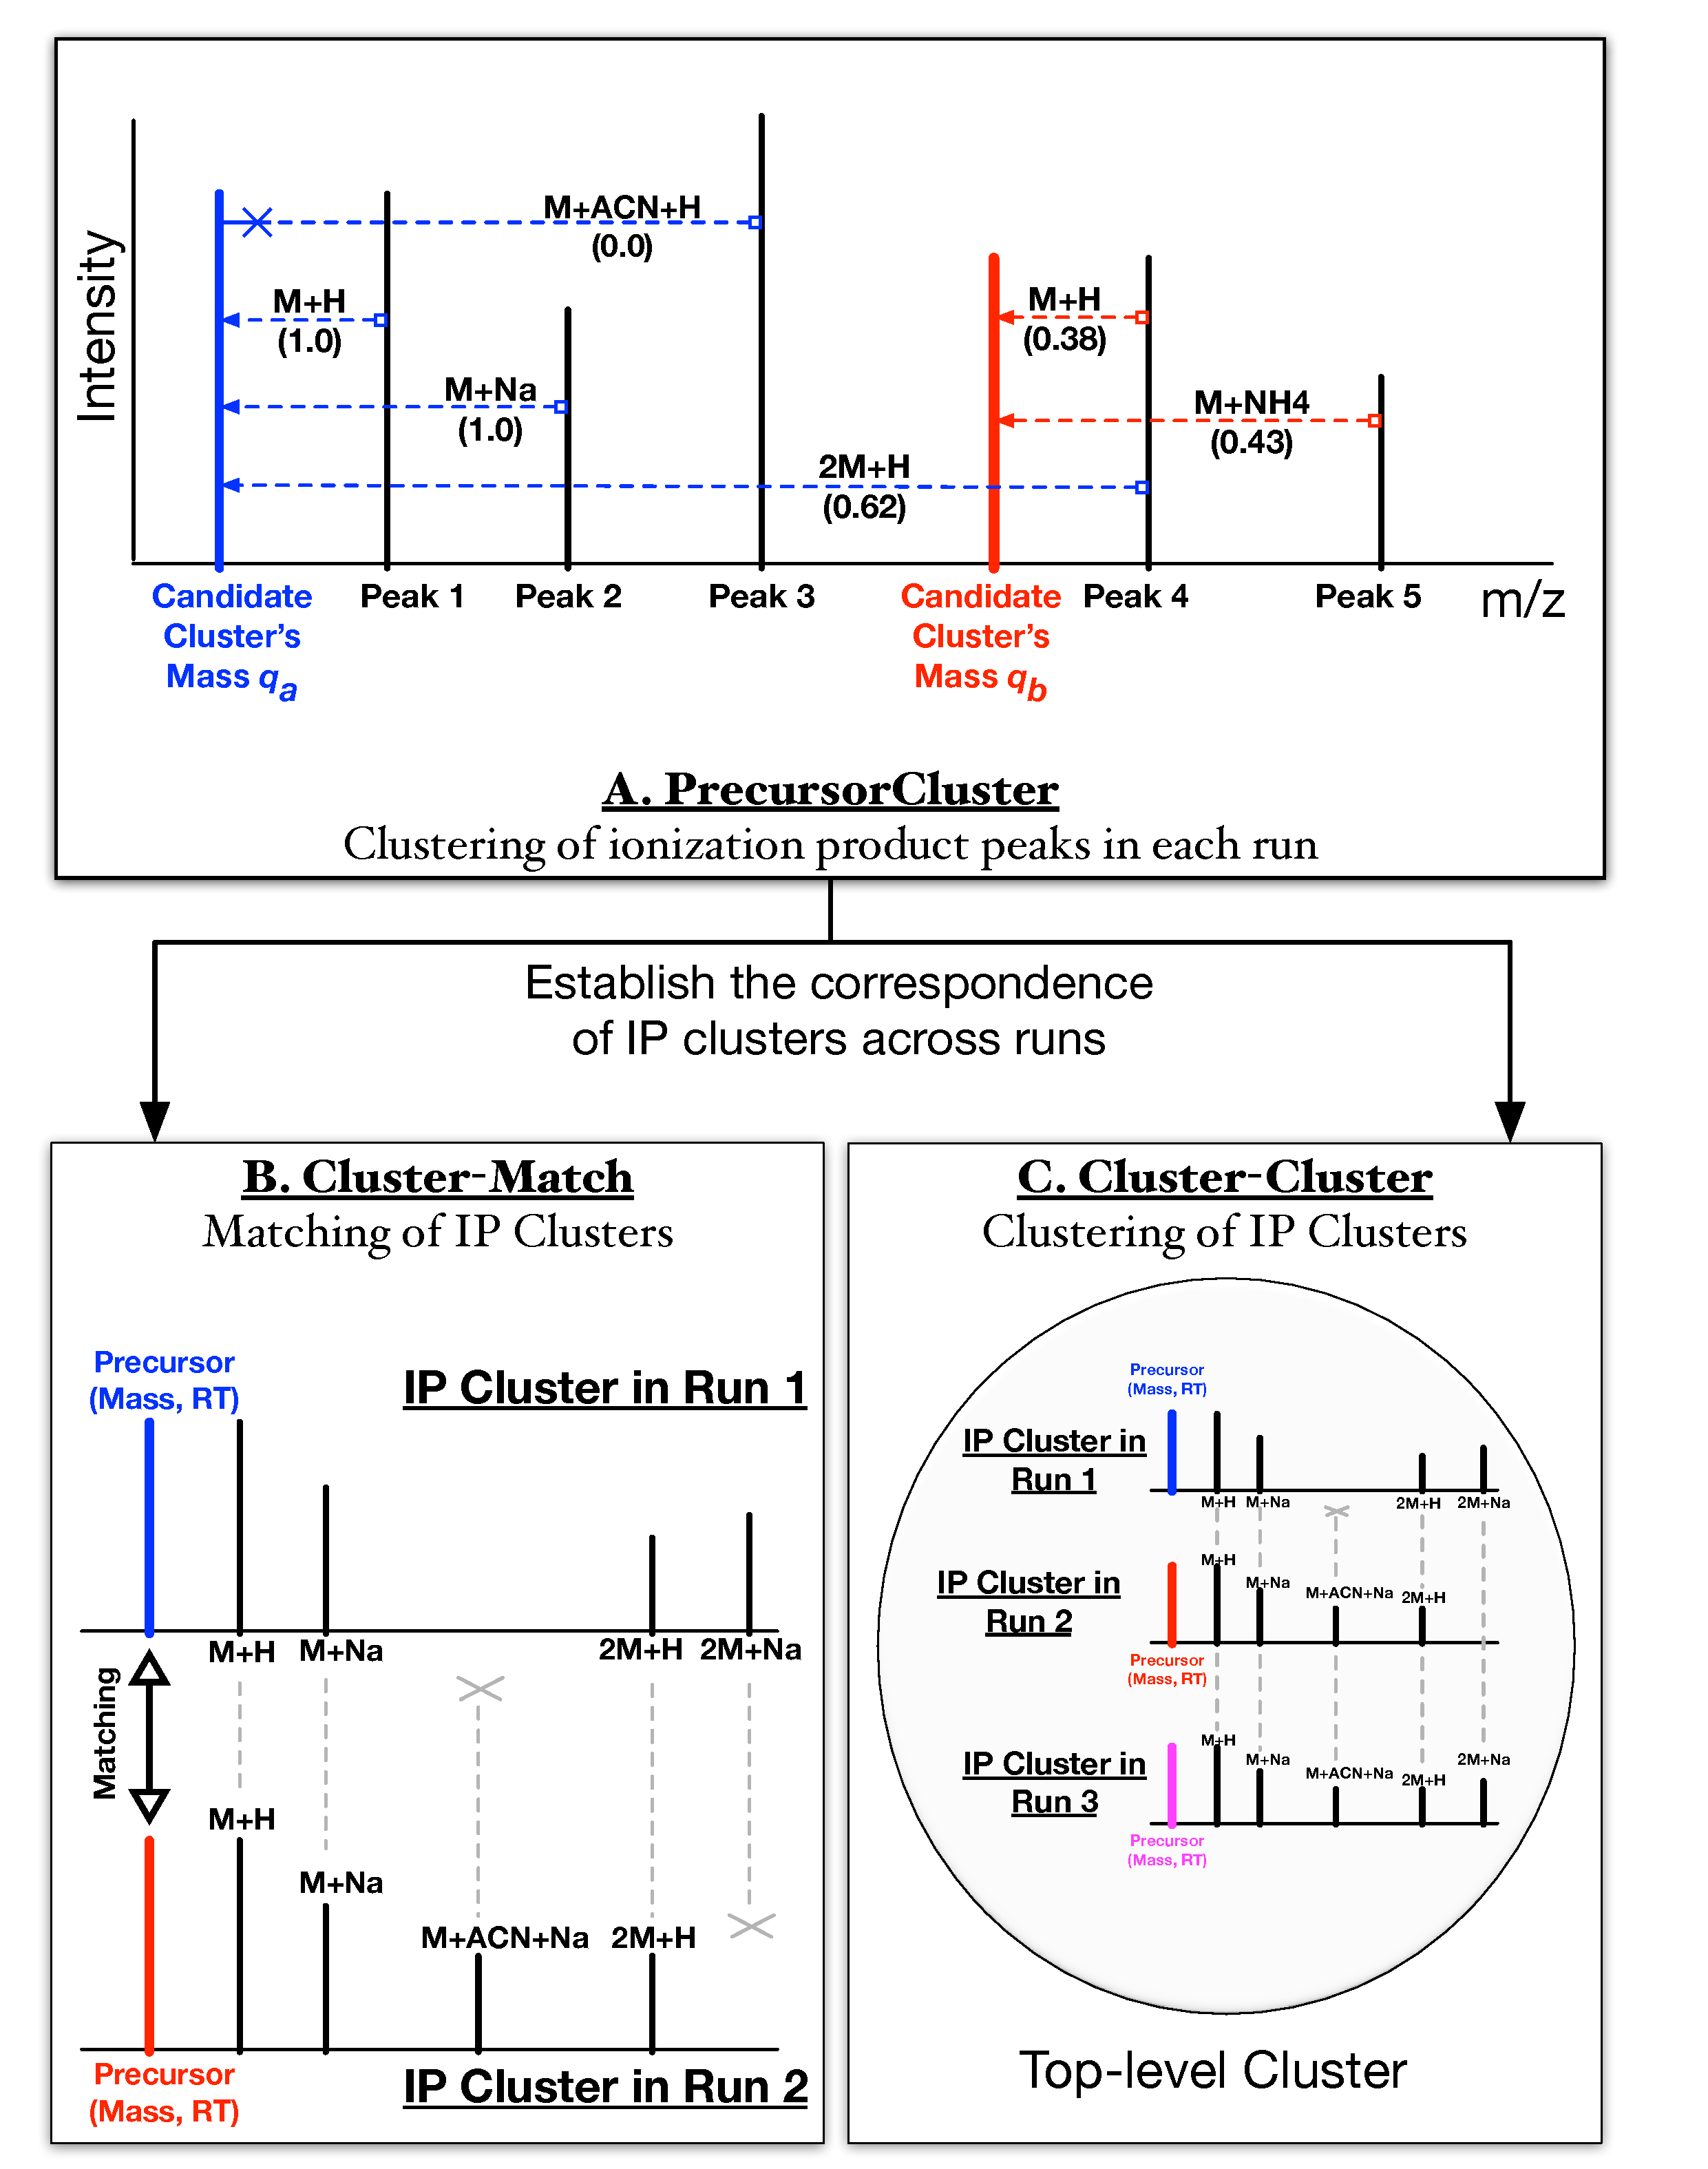
\includegraphics[width=0.5\linewidth]{05-precursor-cluster/figures/fig1.pdf}
\caption{\label{fig:01} An illustration of the proposed methods. The results from inference on the PrecursorCluster model are the set of peaks and their assignments to IP clusters through any of the predefined list of transformation (Fig.~\ref{fig:01}A). As a starting point, each observed peak feature generates a candidate IP cluster, having the cluster's mass computed through the M+H transformation of the observed peak's m/z value. In Fig.~\ref{fig:01}A, this results Peak 1 generating the candidate cluster with mass $q_a$ Peak 4 generating the candidate cluster with mass $q_b$ (other candidate IP clusters produced by Peak 2, 3 and 5 are not shown in the figure). As a result from inference, Peak 1 and Peak 2 are clustered to $q_a$ through the transformation types M+H and M+Na respectively with probability 1.0. Peak 3 has a valid transformation path to $q_a$, but it is not allowed to join that cluster since its intensity is greater than the intensity of the precursor peak. Peak 4 can either form a cluster with $q_a$ through the 2M+H transformation (with probability 0.62) or, through the M+H transformation on itself, form its own candidate IP cluster having the precursor mass $q_b$ (with probability 0.38.) The latter allows for Peak 5 to join that cluster too through the M+NH4 transformation with probability 0.43. For alignment, the final clustering result is established by taking the assignment that has the highest probability for each peak feature. Alignment of IP clusters can be performed by matching IP clusters according to their posterior precursor mass and RT values across runs (Fig.~\ref{fig:01}B) or by further clustering them into top-level clusters in a second-stage clustering process (Fig.~\ref{fig:01}C). The matching of peak features of IP clusters into the same top-level cluster is constructed by matching peak features that have the same transformation types together. These are shown as the gray dotted lines in Figures~\ref{fig:01}B \& C.}
\end{figure}

\subsection{PrecursorCluster: clustering of ionization product peaks\label{sub:ip-clustering}}

A metabolite having a given precursor peak with mass $M$ will be observed as multiple ionization products, including adduct and isotope peaks. For example, rather than measuring the precursor peak with mass $M$, we might measure several IP peaks having the ion masses $[M+H]^+$, $[M+K]^+$ or $[M+ACN+H]^+$. The first-stage clustering model introduced here allows us to perform the grouping of these ionization product peaks generated from the same metabolite. The clustering model takes the form of a mixture model with finite mixture components. 

Within a single run to be processed, we denote its $n$-th peak feature as $\textbf{d}_n$, where $\boldsymbol{d}_n=(m_n,t_n,p_n)$ with $m_n$ the m/z value, $t_n$ the RT value and $p_n$ the intensity value of that peak feature. Assuming that the data is in positive ionization mode (as what we will do throughout this paper) and given a list of $T$ transformations of commonly-known IP types (e.g. M+H, M+2H, 2M+Na), an observed ion peak can possibly be assigned to an IP cluster $k$ only if the peak's ionized m/z value $m_n $ can be transformed through a transformation $u_k$ to a precursor mass $u_k(m_n)$ that falls within a certain user-defined tolerance $\gamma_m$ parts-per-million (ppm) from the precursor mass of the IP cluster. The transformation $u_k$ of the observed mass of peak $n$ to the precursor mass of a cluster $k$ takes the form of $u_k(m_n) = \frac{m_n|c|+ce-\sum_{i} h_i G_i}{m}$, where $c$ is the charge, $e$ is the mass of an electron and $h_i$ and $G_i$ are the atomic masses of adduct parts. Using the adduct transformation M+H+2NA for positive ionization mode data as an example, $c$ is 3, $m$ is 1 while $\sum_{i} h_i G_i$ is the total atomic mass of $H+2Na$. 

Through the M+H transformation, each observed peak produces a candidate IP cluster (corresponding to a mixture component in the model)  This follows from our assumption that for a candidate IP cluster to be considered valid, it must contain the $[M+H]^+$ ion peak that is also the most intense peak in that cluster. Each candidate $k$-th IP cluster now has a tuple of three values associated to it: ($q_k$, $r_k$, $s_k$) where the cluster's mass center $q_k$ is produced by computing the transformed precursor mass under the most common IP type M+H from each observed ion mass in the data, while the cluster's RT center $r_k$ and the cluster's intensity threshold $s_k$ respectively are the RT and intensity values of the ion peak that produces this cluster through the M+H transformation. 

As the next step, we enumerate for each observed peak in the entire run which candidate IP clusters it can possibly be assigned to and through which chemical transformations. As constraints during the enumeration step, an assignment of peak $n$ to candidate cluster $k$ is possible only if \textbf{(1)} the m/z value of that peak can be transformed through any of the $T$ transformations into a precursor mass value that is within $\gamma_m$, the tolerance in parts-per-million (ppm), from the cluster's precursor mass $q_k$, \textbf{(2)} the RT value of that peak is within a certain tolerance ($\gamma_t$ seconds) from the cluster's RT $r_k$ and \textbf{(3)} the intensity of that peak is less than the cluster's intensity $s_k$. These constraints follow from the modelling assumptions that ionization product peaks should co-elute together, having similar RT values to its precursor peak, and the $[M+H]^+$ peak is also the most intense member peak of that IP cluster. The last constraint on intensity helps in obtaining precursor clustering results that are more consistent across runs, but it is not mandatory and can be relaxed if desired. From this enumeration process, it follows that an observed ion peak always satisfies all the constraints of its own IP cluster through the M+H transformation and thus can belong to at least one IP cluster (its own). In dealing with multiple runs, this enumeration process can be performed iteratively for each run being processed or even run in parallel since they are completely independent of each other. 

After enumeration, peaks may have multiple possible candidate IP clusters that they can join through the different transformation types. We use the indicator variable $\boldsymbol{z}_{nk}$ to denote the possible assignment of peak feature $n$ to cluster $k$. Here, $\boldsymbol{z}_{nk}$ is 1 if peak $n$ is assigned to cluster $k$ and 0 otherwise, and each peak can only be assigned to exactly one cluster ($\sum_{k=1}^{K} \boldsymbol{z}_{nk}=1$). We can model $\boldsymbol{z}_{n}$ as a multinomial distribution having the parameter vector $\boldsymbol{\theta}$, itself drawn from a prior Dirichlet distribution having the symmetric parameter $\alpha$. The likelihood of a peak $n$ to be assigned to a possible cluster $k$ depends on the likelihood of that peak's transformed precursor mass and RT values under the cluster's mass and RT centers. The complete model for the clustering of ionization product peaks is therefore:
\begin{align} 
\boldsymbol{\theta}\vert\alpha &\sim Dir(\alpha) \\
\boldsymbol{z}_n\vert\boldsymbol{\theta} &\sim Multinomial(\boldsymbol{\theta}) \\
\boldsymbol{d}_n\vert\boldsymbol{z}_{nk}=1,... &\sim L(\boldsymbol{d}_n\vert\boldsymbol{z}_{nk}=1,...)
\end{align}
where $L(\boldsymbol{d}_n\vert\boldsymbol{z}_{nk}=1,...)$ is the likelihod of peak $n$ under cluster $k$ and $...$ is to denote any other parameters being conditioned upon but not explicitly listed to the right of the conditioning bar. Assuming that the likelihood term in eq. (3) can be factorized into independent mass and RT terms, we get:
\begin{equation}
L(\boldsymbol{d}_n\vert\boldsymbol{z}_{nk}=1,...)=p(u_k(m_n)\vert\boldsymbol{z}_{nk}=1,...) \cdot p(t_n\vert\boldsymbol{z}_{nk}=1,...)
\end{equation}
For the mass term $p(u_k(m_n)\vert\boldsymbol{z}_{nk}=1,...)$ in eq. (4), the likelihood of the transformed precursor mass $u_k(m_n)$ is a product of two further terms, shown in eq. (5). The first is the indicator function $I(u_k)$, set to 1 if there are no other peaks assigned to cluster $k$ through transformation $u_k$, and 0 otherwise. This allows each transformation type to only appear once in each IP cluster. Next, the transformed precursor mass $u_k(m_n)$ is distributed according to a Gaussian distribution with mean equal to the cluster mass center $q_k$ and precision (inverse variance) of $\delta$. We set $\delta$ to reflect the mass tolerance in parts-per-million used during the enumeration of possible assignments of peaks to potential IP clusters, such that one standard deviation ($\sqrt{\delta^{-1}}$) is set to be $\frac{\gamma_m*q_k/1e6}{3}$. The cluster mass center $q_k$ is in turn drawn from a prior Gaussian distribution having prior mass mean $\mu_0$ and precision $\delta$. Since the prior value of the cluster mass mean $q_k$ is pretty constrained and cannot deviate far from the transformed $[M+H]^+$ mass value, it makes sense to set $\mu_0=q_k$ in the prior distribution for $q_k$ in eq. (6).
\begin{align}
p(u_k(m_n)\vert\boldsymbol{z}_{nk}=1,q_k,\delta,...) &\sim I_k(n) \cdot \mathcal{N}(u_k(m_n) \vert q_k,\delta^{-1}) \\
p(q_k\vert \mu_0,\delta) &\sim \mathcal{N}(q_k \vert \mu_0,\delta^{-1})
\end{align}

Similarly for the RT term $p(t_n\vert\boldsymbol{z}_n=k,...)$ in eq. (4), the RT value $t_n$ is distributed according to the Gaussian distribution having mean the cluster RT center $q_k$ and precision $\lambda$ set to reflect the RT tolerance used during enumeration of possible assignments, i.e. $\gamma_t$ is $3\sqrt{\lambda^{-1}}$. The cluster RT center $r_k$ is drawn from a prior Gaussian distribution with mean $\psi_0$ (set to be the same as $r_k$ itself) and precision $\lambda$.
\begin{align}
p(t_n\vert\boldsymbol{z}_{nk}=1,r_k,\lambda) &\sim \mathcal{N}(t_n \vert r_k,\lambda^{-1}) \\
p(r_k\vert \psi_0,\lambda) &\sim \mathcal{N}(r_k \vert \psi_0,\lambda^{-1})
\end{align}

Given the complete specifications of the model in eq. (1-8), our goal is to infer $\boldsymbol{z}_{nk}$, the assignments of peak $n$ to possible cluster $k$. A Gibbs sampling scheme \cite{Rogers2011} is used to approximate the joint distribution of the model during inference 
\todo[inline]{Add Gibbs sampling details for PrecursorCluster}

Once Gibbs sampling has finished and enough posterior samples have been collected, peaks are then assigned to the most likely IP cluster based on their \textit{maximum a-posteriori} probabilities averaged across the samples obtained from Gibbs sampling after ensuring convergence. The final result from inference is the set of IP clusters, some of which may be empty and can be ignored while others consist of the observed peak that can be transformed into that cluster's precursor mass through the M+H transformation, alongside with other peaks that can be related to the precursor mass through the set of transformations defined by the user. Additionally, for each IP cluster, we also compute the precursor peak's mass and RT values from the posterior distributions of those parameters. These will be useful in the latter stages of matching IP clusters across runs.

\subsection{Cluster-Match: direct matching of ionization product clusters\label{sub:cluster-match}}

The ionization product clustering model described in Section~\ref{sub:ip-clustering} is essentially a data-reduction procedure, where within a single file $j$, the model takes as input the set of observed peaks in a single run and produces as output their groupings into IP clusters. Given the set of non-empty IP clusters and the peak features they contain, we can now treat IP clusters as a reduced set of features within a run and align (match) them across runs. We call this approach Cluster-Match. This contrasts to the conventional approach of matching all peak features directly to produce the alignment of peak features across runs. 

The results from inference in Section~\ref{sub:ip-clustering} is the assignment of peaks to their most likely clusters, alongside the annotation of the most likely transformation type that brings the peaks into an IP cluster. Specifically for the purpose of matching, each cluster $k$ in file $j$ is now associated to $\boldsymbol{c}_{jk}$, where $\boldsymbol{c}_{jk}=({\bar{q}}_{jk}, {\bar{r}}_{jk})$. Here, ${\bar{q}}_{jk}$ is the posterior precursor mass value for that cluster, which takes into account the prior probability on the mass and also the transformed precursor masses of observed peaks assigned to it. Similarly, ${\bar{r}}_{jk}$ is the posterior RT value for cluster $k$ in file $j$. The same procedure used for matching peak features across runs can now be used to match IP clusters across runs and is briefly summarized in the following paragraph.

As detailed in Chapter~\ref{c:matching}, in the direct matching alignment of two runs, the problem of establishing the matching between two runs can be viewed as finding the maximum weighted matching in a bipartite graph, where a node in the graph represents a peak feature, an edge represents a potential matching across two sides of the graph and the edge weight is the similarity between two potential matches. The MW method  in Chapter~\ref{c:matching} is an instance of a greedy algorithm that produces an approximation of at least 1/2 of the maximum weight in the matching of a bipartite graph \cite{Maximum2011}. Only peaks that are within mass and RT tolerances from each other across runs can possibly be matched (they have an edge linking them in the graph). While simple, the results in Chapter~\ref{c:matching} shows that the MW method is generally competitive in performance to more sophisticated direct-matching methods, such as SIMA that relies on constructing stable-matching. We apply this direct matching methods to match IP clusters across runs, with IP clusters taking the place of individual peak features as nodes in the bipartite graph to be matched. The matching is therefore performed based on the precursor mass and RT values of IP clusters, rather than the observed peak's m/z and RT values. Once matching has been constructed, the alignment between the actual peak features in matched IP clusters can be established by grouping peaks that have the same transformation type across matched IP clusters (Figure~\ref{fig:01}B.)

To extend the above procedure to the alignment of multiple runs, two initial runs are first aligned to construct an intermediate merged results. Consensus features are created by taking the average m/z and RT values of matched features, and the next run is then aligned to the merged results. This procedure is repeated until all runs have been exhausted. This match-merge scheme is commonly employed by other direct matching methods \cite{Voss2011a, Pluskal2010} and requires selecting a reference run. In practice, the choice of reference run is arbitrary and its effect has not been fully investigated (in our implementation, the first run in alphabetical sorting is used as the reference run and the same ordering of runs is always used for all methods compared.)

\subsection{Cluster-Cluster: across-run clustering of ionization product clusters\label{sub:cluster-cluster}}

The proposed pairwise matching scheme used by Cluster-Match is frequently extended to the processing of multiple runs in a fairly ad-hoc manner (as seen in the match-merge approach at the end of Section~\ref{sub:cluster-match}, also commonly used by other direct matching tools). This approach suffers from the limitation of having to set a reference run for the matching and consequently, the fact that altering the ordering of runs to be processed might change the alignment results \cite{Smith2013}. The alternative approach of generalizing from pairwise matching in a bipartite graph into finding the maximum weighted matching in a general graph is typically a computationally expensive operation. Producing a distance measure that works well for measuring similarities of peaks across runs is a non-trivial problem, and such matching procedures, whether through successive pairwise merging or operating on a general graph, generally do not take into account the uncertainties in the matching of peak features across runs.

Here, we propose using another clustering procedure (Cluster-Cluster) to further cluster the IP clusters produced from the first-stage IP clustering in Section~\ref{sub:ip-clustering}. In this manner, IP clusters coming from different runs are further clustered into top-level clusters shared across runs (Figure~\ref{fig:01}C). The actual alignment of peak features can then be established by \textbf{(1)} looking at which IP clusters are put together into the same top-level cluster (essentially, their matching) and \textbf{(2)} in a top-level cluster, grouping peak features from different runs that have the same transformation type together to establish their alignments. Crucially, the posterior probabilities of certain IP clusters being assigned into the same top-level cluster provides us with an estimate of matching confidence of peak features.

As only peaks that are within a certain mass tolerance (which depends on the instrument's accuracy) should be matched across runs, we perform a preliminary partitioning of IP clusters based on their posterior precursor mass values into top-level mass bins. $\gamma'_m$ is defined to be the across-run mass tolerance threshold used for the pre-grouping IP clusters coming from different runs. Across all runs $j=1,...,J$, IP clusters are first sorted by their posterior mass values $\{{\bar{q}}_{jk}\}$. The smallest mass value $min(\{{\bar{q}}_{jk}\})$ is used to group other IP clusters into the top-level bin. Grouping is done in successive ascending mass order until the next IP cluster to be grouped has the posterior mass value that differs by $\gamma'_m$ ppm from $min(\{{\bar{q}}_{jk}\})$. In this case, a new top-level bin is started and the next ungrouped mass value is used for the grouping of the remaining other peaks. This procedure is repeated until all peaks have been exhausted.

Within a top-level mass bin, we now have IP clusters coming from different runs having similar posterior mass values but potentially different posterior RT values and member peaks. For each $k$-th IP cluster coming from file $j$, an adduct `fingerprint' vector $\boldsymbol{\bar{u}}_{jk}$ of length $T$ is created after the MAP assignment of observed peaks into the IP cluster. $\boldsymbol{\bar{u}}_{jk}$ stores the information on which adduct transformations bring member peaks into that IP cluster, with the corresponding entry in $\boldsymbol{u}_{jk}$ set to 1 if that transformation exists and 0 otherwise. Let $y_i$ be the list of IP clusters coming from different runs that have been pre-grouped in a top-level mass bin $i$, i.e. $y_i=(\boldsymbol{c}_{jk},...)$ where $\boldsymbol{c}_{jk}=({\bar{q}}_{jk}, {\bar{r}}_{jk}, \boldsymbol{\bar{u}}_{jk})$. Here, ${\bar{q}}_{jk}$ is the IP cluster's posterior mass value, ${\bar{r}}_{jk}$ the posterior RT value and $\boldsymbol{\bar{u}}_{jk})$ the adduct fingerprint of that IP cluster. If the top-level mass bin contains only 1 IP cluster, no possible matching can be constructed. In the case of more than 1 IP clusters present in a top-level bin, the IP clusters that have similar posterior mass and RT values and adduct fingerprints can be grouped together into a top-level cluster. To avoid specifying the number of top-level clusters \textit{a priori}, we use an infinite Gaussian mixture model, described in Chapter~\ref{c:ml-background} to model the data. 

Let the indicator $\boldsymbol{\bar{z}}_{jki}=1$ denotes the assignment of IP cluster $k$ coming from file $j$ into top-level cluster $i$. Then:
\begin{align}
\boldsymbol{\pi}\vert\alpha' &\sim GEM(\alpha') \\
\boldsymbol{\bar{z}}_{jk}\vert\boldsymbol{\pi} &\sim Multinomial(\boldsymbol{\pi}) \\
\boldsymbol{c}_{jk}\vert\boldsymbol{\bar{z}}_{jki}=1,... &\sim L(\boldsymbol{c}_{jk}\vert\boldsymbol{\bar{z}}_{jki}=1,...)
\end{align}
where $\boldsymbol{\pi}$ is the mixing proportions, now distributed according to the GEM (Griffiths, Engen and McCloskey) distribution (details in the Supplementary). In this model, the number of mixture components and the sparsity of each component depends on the concentration hyper-parameter $\alpha'$. Next, the likelihood of $\boldsymbol{c}_{jk}$ (the $k$-th IP cluster from run $j$) to be in a top-level cluster $i$ is assumed to be factorized into independent factors of its mass, RT and adduct signature terms:
\begin{equation}
\begin{split}
L(\boldsymbol{c}_{jk}\vert\boldsymbol{\bar{z}}_{jki}=1,...) = p({\bar{q}}_{jk}\vert\boldsymbol{\bar{z}}_{jki}=1,...) \cdot p({\bar{r}}_{jk}\vert\boldsymbol{\bar{z}}_{jki}=1,...) \cdot \\
p({\boldsymbol{\bar{u}}}_{jk}\vert\boldsymbol{\bar{z}}_{jki}=1,...)
\end{split}
\end{equation}
In this likelihood of eq. (12), the mass term $p({\bar{q}}_{jk}\vert\boldsymbol{\bar{z}}_{jki}=1,...)$ is defined analogously to the first-stage clustering in Section~\ref{sub:ip-clustering}. First, we have the indicator function $\bar{I}(jki)$ set to 1 if there are no other IP clusters from run $j$, apart from the $k$-th IP cluster in $j$, that are assigned to the $i$-th top-level cluster, and 0 otherwise. This ensures that there is only most one IP cluster from each run assigned to a top-level cluster. Next, the IP cluster posterior mass ${\bar{q}}_{jk}$ is distributed according to a Gaussian distribution with mean $c_m$ and precision $\bar{\delta}$, where the across-run mass tolerance $\gamma'_m$ is set to be equivalent to 3 standard deviations in ppm. The cluster mass center $c_m$ is in turn drawn from a base Gaussian distribution having prior mass mean $\bar{\mu}_0$ and precision $\sigma_m$. We set $\bar{\mu}_0$ to the mean of the posterior m/z values of the IP clusters in the top-level bin, while $\sigma_m$ is set to a broad value of 5E-3. 
\begin{align}
p({\bar{q}}_{jk}\vert\boldsymbol{z}_{jki}=1,c_m,\bar{\delta},...) &\sim \bar{I}(jki) \cdot \mathcal{N}(\bar{q}_{jk} \vert c_m,\bar{\delta}^{-1}) \\
p(c_m\vert \bar{\mu}_0,\sigma_m) &\sim \mathcal{N}(c_m \vert \bar{\mu}_0,\sigma_m^{-1})
\end{align}
Similarly, in the RT term $p({\bar{r}}_{jk}\vert\boldsymbol{z}_{jki}=1,...)$, ${\bar{r}}_{jk}$ is distributed according to a Gaussian distribution with mean $c_t$ and precision $\bar{\lambda}$. Again, the across-run RT tolerance $\gamma'_t$ set to be equivalent to 3 standard deviations in seconds. The same uninformative parameter values are set on the prior RT mean parameter $\bar{\psi}_0$ and precision $\sigma_t$.
\begin{align}
p({\bar{r}}_{jk}\vert\boldsymbol{z}_{jki}=1,c_t,\bar{\lambda}) &\sim \mathcal{N}({\bar{r}}_{jk} \vert c_t,\bar{\lambda}^{-1}) \\
p(c_t\vert \bar{\psi}_0,\sigma_t) &\sim \mathcal{N}(c_t \vert \bar{\psi}_0,\sigma_t^{-1})
\end{align}
Finally, in the adduct fingerprint term $p({\boldsymbol{\bar{u}}}_{jk}\vert\boldsymbol{z}_{jki}=1,...)$, the vector ${\boldsymbol{\bar{u}}}_{jk}$ is modelled using a multinomial distribution having a Dirichlet prior with symmetric hyper-parameter $\beta$.  The use of multinomial distribution here to model the binary vector ${\boldsymbol{\bar{u}}}_{jk}$ provides a flexibility to the Cluster-Cluster model, should the constraint of having each transformation type appear at most once in each IP cluster is removed from the first-stage clustering step.

\begin{align}
\boldsymbol{\psi}\vert\beta &\sim Dir(\beta) \\
{\boldsymbol{\bar{u}}}_{jk}\vert\boldsymbol{\psi} &\sim Multinomial(\boldsymbol{\psi})
\end{align}
Taken together, the entire likelihood function of eq. 12 ensures that IP clusters coming from different runs can only be put together in a single top-level cluster if: \textbf{(1)} they come from different runs, \textbf{(2)} they share similar posterior precursor mass and RT values, and \textbf{(3)} they have similar adduct fingerprint. Inference on model parameters is again performed via Gibbs sampling. Within each sample, we establish the alignments of peaks in matched IP clusters by grouping peaks with the same transformation type together (Figure~\ref{fig:01}C), forming aligned peaksets. The occurrences of aligned peaksets are counted and averaged across samples to get the estimate of matching confidence. 

\todo[inline]{Add Gibbs sampling details for Cluster-Cluster}

\section{Evaluation Study}

\subsection{Evaluation Datasets}

We evaluated the performance of the proposed alignment methods on two metabolomic datasets. The first dataset is generated from a mixture of 104 standard metabolites used for the calibration of chromatographic columns, labelled the Standard dataset and is available in 11 runs in total. Alongside its associated alignment ground truth, the Standard dataset has been used for performance evaluation of alignment methods in Chapter~\ref{c:matching}. While the runs are not true technical replicates, they are similar enough to be treated as replicates for the purpose of performance evaluation. Indeed the Standard runs represent a fairly challenging alignment scenario due to the variability in the RT values of peak features as the runs were produced from different LC-MS analyses separated by weeks and on different instruments.

Additionally, in this paper, we also introduce a new dataset obtained from sampling a bottle of `Seven Giraffes Extraordinary Ale'. This Beer dataset is available in 3 runs. While the Beer runs have minimal RT deviations, it is fairly is representative of the typical biochemical diversity in a complex metabolomics study and can provide a useful portrayal on how the evaluated methods might perform in real-life usage. A Thermo Scientific Ultimate 3000 RSLCnano liquid chromatography system (Thermo Scientific, CA, USA) was coupled to a Thermo Scientific Q-Exactive Orbitrap mass spectrometer equipped with a HESI II interface (Thermo Scientific, Hemel Hempstead, UK). The HILIC separation was performed with a SeQuant ZIC- pHILIC column (150 x 4.6 mm, 5 μm) equipped with the corresponding pre-column (Merck Sequant, Darmstadt, Germany). ACN buffer and H$_2$O with amonium carbonate were used in the chromatography.

\subsection{Performance Measures}

The different alignment methods being compared return as results the matchings of peak features coming from different runs. In the case of Cluster-Cluster, such aligned peaksets also have probability values, potentially corresponding to matching confidence, attached to them. To evaluate alignment results on multiple runs, we propose generalizing the pairwise performance measures outlined in the previous Chapter~\ref{c:matching} to the alignment of multiple runs. Performance of the evaluated methods is still quantified in terms of precision and recall. `Precision' here refers the fraction of aligned peaksets returned by a method that are relevant (in accordance to some alignment ground truth), while `recall' refers the fraction of relevant aligned peaksets that are returned by an alignment method. 

To provide a definition of `precision' and `recall' suitable for evaluating alignment performance, we begin by enumerating all the possible $l$-size combinations for every aligned peakset in both the method's output and the ground truth list. For example, an alignment method returns a list of two aligned peaksets $\{a,b,c,d,\},\allowbreak\{e,f,g\}$ as output. When $l=2$, this output can be enumerated into a list of 9 `alignment items' of all the pairwise combinations of features: $\{a,b\},\allowbreak\{a,c\},\allowbreak\{a,d\},\allowbreak\{b,c\},\allowbreak\{b,d\},\allowbreak\{c,d\},\allowbreak\{e,f\},\allowbreak\{e,g\},\allowbreak\{f,g\}$. Let $M$ and $G$ be the results from such enumeration from a method's output and the ground truth respectively. Each distinct combination of features in $M$ and $G$ can be considered as an item during performance evaluation. Intuitively, the choice of $l$ reflects the strictness of what is considered to be a true positive item, with larger values of $l$ demanding an alignment method that produces results spanning more runs correctly. In this manner, $l$ goes from 2 to as many runs being aligned.

For a given $l$, the following positive and negative instances of alignment item can now be defined for the purpose of performance evaluation:
\begin{itemize}
\item True Positive ($\boldsymbol{TP}$): items that should be aligned (present in $G$) and are aligned (present in $M$).
\item False Positive ($\boldsymbol{FP}$): items that should not be aligned (absent from $G$) but are aligned (present in $M$).
\item True Negative ($\boldsymbol{TN}$): items that should not be aligned (absent from $G$) and are not aligned (absent from $M$).
\item False Negative ($\boldsymbol{FN}$): items that should be aligned (present in $G$) but are not aligned (absent from $M$).
\end{itemize}

In the context of alignment performance, precision ($\frac{\boldsymbol{TP}}{\boldsymbol{TP}+\boldsymbol{FP}}$) is therefore the fraction of alignment items in $M$ that are correct with respect to some alignment ground truth $G$, while recall ($\frac{\boldsymbol{TP}}{\boldsymbol{TP}+\boldsymbol{FN}}$) is the fraction of alignment items specified in $G$ that are actually aligned in the alignment results $M$. By definition, a perfect alignment method would have precision and recall scores of 1. In practice, there is a trade-off between precision and recall, where increasing recall often results in lower precision and vice versa. To summarize these two numbers, we also report the F$_1$ score, which is the harmonic mean of precision and recall, defined as $F_1 = 2(precision\cdot recall)/(precision + recall)$. Since our alignment ground truth is usually smaller than the set of all pairs of peaks returned by a method, only those peaks present in the ground truth are considered for evaluation. 

\subsection{Evaluation Procedure\label{sub:evaluation_procedure}}

As the baselines for evaluation, we compare the performance of our proposed methods against the method of direct matching of peak features (MW) and its variant (MWG) that modifies the similarity matrix used during matching to bring together group of peaks related by RT closer during matching -- described in Chapter~\ref{c:matching}. 

To evaluate Cluster-Match, we followed the experimental procedure in Chapter~\ref{c:matching}. 30 random pairs of runs were selected from the Standard runs and designated as the Standard training set, and another 30 pairs of runs selected as the Standard testing set. Each run is then processed through the first-stage ionization product clustering (PrecursorCluster) using the same set of parameters, as detailed in Section~\ref{sub:parameters}. Matching tolerance parameters were varied within reasonable ranges on one pair in the training set (see Section~\ref{sub:parameters} for details) and parameters that result in the best training performance, i.e. highest $F_1$-score, were then applied onto its associated pair in the testing set. Measuring performance on a different testing set provide us with a picture on how the methods being evaluated generalize to new data in actual usage. The number of available 3 Beer runs is too few to allow separation of the runs into training and testing sets, so the 3 beer runs were used at once for performance evaluation. For each method, we report the results obtained from all combinations of parameters being varied on the Beer dataset, i.e. the training results only.

To evaluate Cluster-Cluster, we selected five sets of 2, 3, and 4 Standard runs randomly, and also the same set of 3 Beer runs. All runs have been processed through the PrecursorCluster model. For each data set, parameters for Cluster-Match were varied following see Section~\ref{sub:parameters} to obtain the best attainable alignment performance for comparison. The best results from Cluster-Match are then compared against the output from Cluster-Cluster on the same set of data but using a fixed set of parameters for the second-stage clustering. We also ran Cluster-Cluster with and without the adduct fingerprint term to evaluate the importance of that term to the alignment results of Cluster-Cluster.

\subsection{Parameter Optimization\label{sub:parameters}}

Common to all the direct matching method used in the evaluation study are the m/z and RT window tolerance parameters, which define the maximum deviation acceptable for a candidate matching is allowed in the bipartite graph. The choice of m/z parameter is often determined by the accuracy of the mass spectrometry instrument and can be reasonably determined in advance. Due to RT drift, selecting the RT window is less straightforward. 

On the Standard datasets, we varied the mass tolerance window of the methods tested within the range $\{2, 4, 6, 8, 10\}$ m/z and the RT tolerance window within $\{5, 10, 15, ..., 100\}$ seconds during the training stage. Parameter combinations that result in the best F1-score were then used for performance evaluation in the testing stage. For MWG, additional parameters are also required for the threshold $t_{g}$ on greedy clustering of related peaks and $\alpha_{g}$, the contribution on the different parts to the similarity score (more details in \cite{Wandy2015}). We let $t_g$ vary within $\{2, 4, 6, 8, 10\}$ seconds and $\alpha_g$ within $\{0, 0.2, 0.4, 0.6, 1.0\}$ in the training stage and use the best combinations of parameter values for the testing stage.

The following parameters were used for the first-stage clustering of the PrecursorCluster model for all the Standard runs being processed: within-run mass tolerance $\gamma_m=5$ ppm, within-run RT tolerance $\gamma_t=30$ seconds. For the Beer runs, we used the within-run mass tolerance $\gamma_m=3$ ppm and the within-run RT tolerance $\gamma_t=10$ seconds. The prior on the Dirichlet distribution $\alpha$ is set to 1.0 and Table~\ref{Tab:transformation} shows the list of common adduct transformations in positive ionization mode used for precursor clustering. 5000 posterior samples were obtained from Gibbs sampling.

\begin{table}[!htbp]
\caption{List of common adduct transformations in positive mode used for the precursor clustering of the Standard and Beer runs.\label{Tab:transformation}}{\begin{tabular}{@{}lllll@{}}
M+2H & M+H & M+ACN+H & 2M+Na & M+H+NH4\\
M+NH4 & M+ACN+Na & 2M+ACN+H & M+ACN+2H & M+Na\\
M+2ACN+H & M+2ACN+2H & M+CH3OH+H & 2M+H
\end{tabular}}{}
\end{table}

For the second-stage clustering in Cluster-Cluster, the following parameters were used for all input Standard and Beer runs: across-run mass tolerance $\gamma'_m=10$ ppm, across-run RT tolerance $\gamma'_t=60$ seconds, $\alpha'$ the Dirichlet Process concentration parameter is set to 1000.0 (intuitively, large values of $\alpha'$ will produce more top-level clusters, each having fewer member IP clusters inside), while $\beta$, the symmetric prior on the Dirichlet prior distribution for adduct signature vector is set to 0.1. Inference is performed on each top-level bin that has more than 1 IP clusters inside, with 500 posterior samples drawn for each top-level bin.

\section{Results and Discussions}

With PrecursorCluster, the large number of peaks present within a single LC-MS run can now be reduced to a smaller number of IP clusters, making alignment easier as fewer objects have to be matched across runs. Section~\ref{sub:precursor-cluster-results} presents the results of running the ionization product clustering on the Standard and Beer datasets. 

While the resulting IP clusters potentially have many uses (e.g. to the problem of annotation of related peaks and the identification of metabolites), peaks assigned to any IP cluster have now been annotated with the transformation type that brings them into the clusters. IP clusters can therefore be aligned across runs (through direct-matching or a second-stage clustering process) and their member peak features (sharing the same transformation type) matched to produce alignment. Section~\ref{sub:cluster-match-results} demonstrated from our experiments how the proposed approach of direct-matching IP clusters can improve upon the matching of LC-MS peak features alone, while Section~\ref{sub:cluster-cluster-results} describes how the resulting probabilities from Cluster-Cluster can be used to robustly quantify the matching uncertainties.

Being a direct matching method, Cluster-Match performs nearly as fast as alignment by matching of peak features alone while offering better performance. As Cluster-Cluster performs Bayesian inference on which IP clusters should be put together into the same top-level clusters, the alignment of LC-MS features can now be established without the need for a reference run. While this requires more computational time than the direct-matching alternative (Section~\ref{sub:running-time}), Cluster-Cluster is able to produce confidence scores on the matching quality of aligned peaksets from the posterior summaries computed during inference. This has a potential use in assisting the selection of high-confident aligned peaksets for subsequent analysis in the latter stage of the LC-MS pipeline

\subsection{Ionization product clustering using PrecursorCluster}

Once PrecursorCluster has been performed on each input file, peaks are MAP-assigned to their respective IP clusters according to the possible transformation types. Table~\ref{Tab:cluster-counts} summarizes the results from PrecursorCluster when only the adduct transformations types, common in positive ionization mode (Table~\ref{Tab:transformation}), are considered. We see from Table~\ref{Tab:transformation} that within each run, a large number of peak features cannot be clustered to other peaks within the same run and can therefore only form an IP cluster with itself as the only member through the M+H transformation (we call these clusters of only one member peak the singleton IP clusters). In both the Standard and Beer runs, non-singleton IP clusters (containing more than one member peaks) comprise approximately 6\% to 10\% of the total IP clusters of that run. The distributions of the cluster sizes of these non-singleton clusters when only adduct transformations are used are given in Figure~\ref{fig:cluster-counts} for the Standard and Beer runs. We also note that for any given cluster size, the counts of IP clusters of that size tend to differ significantly across the Standard runs, due to the varying number of LC-MS peak features present in each Standard run. This is the consequence of the Standard runs being produced in several batches separated over a period of time. The distributions of cluster sizes in Figure~\ref{fig:cluster-counts} across the three Beer runs are more consistently reproduced, reflecting the fact that the runs were generated within the same batch. As shown in Figure~\ref{fig:cluster-counts}, the largest IP clusters of the Beer and Standard runs have 6 and 7 member peaks respectively. 

\begin{figure}[!htbp]
\centering
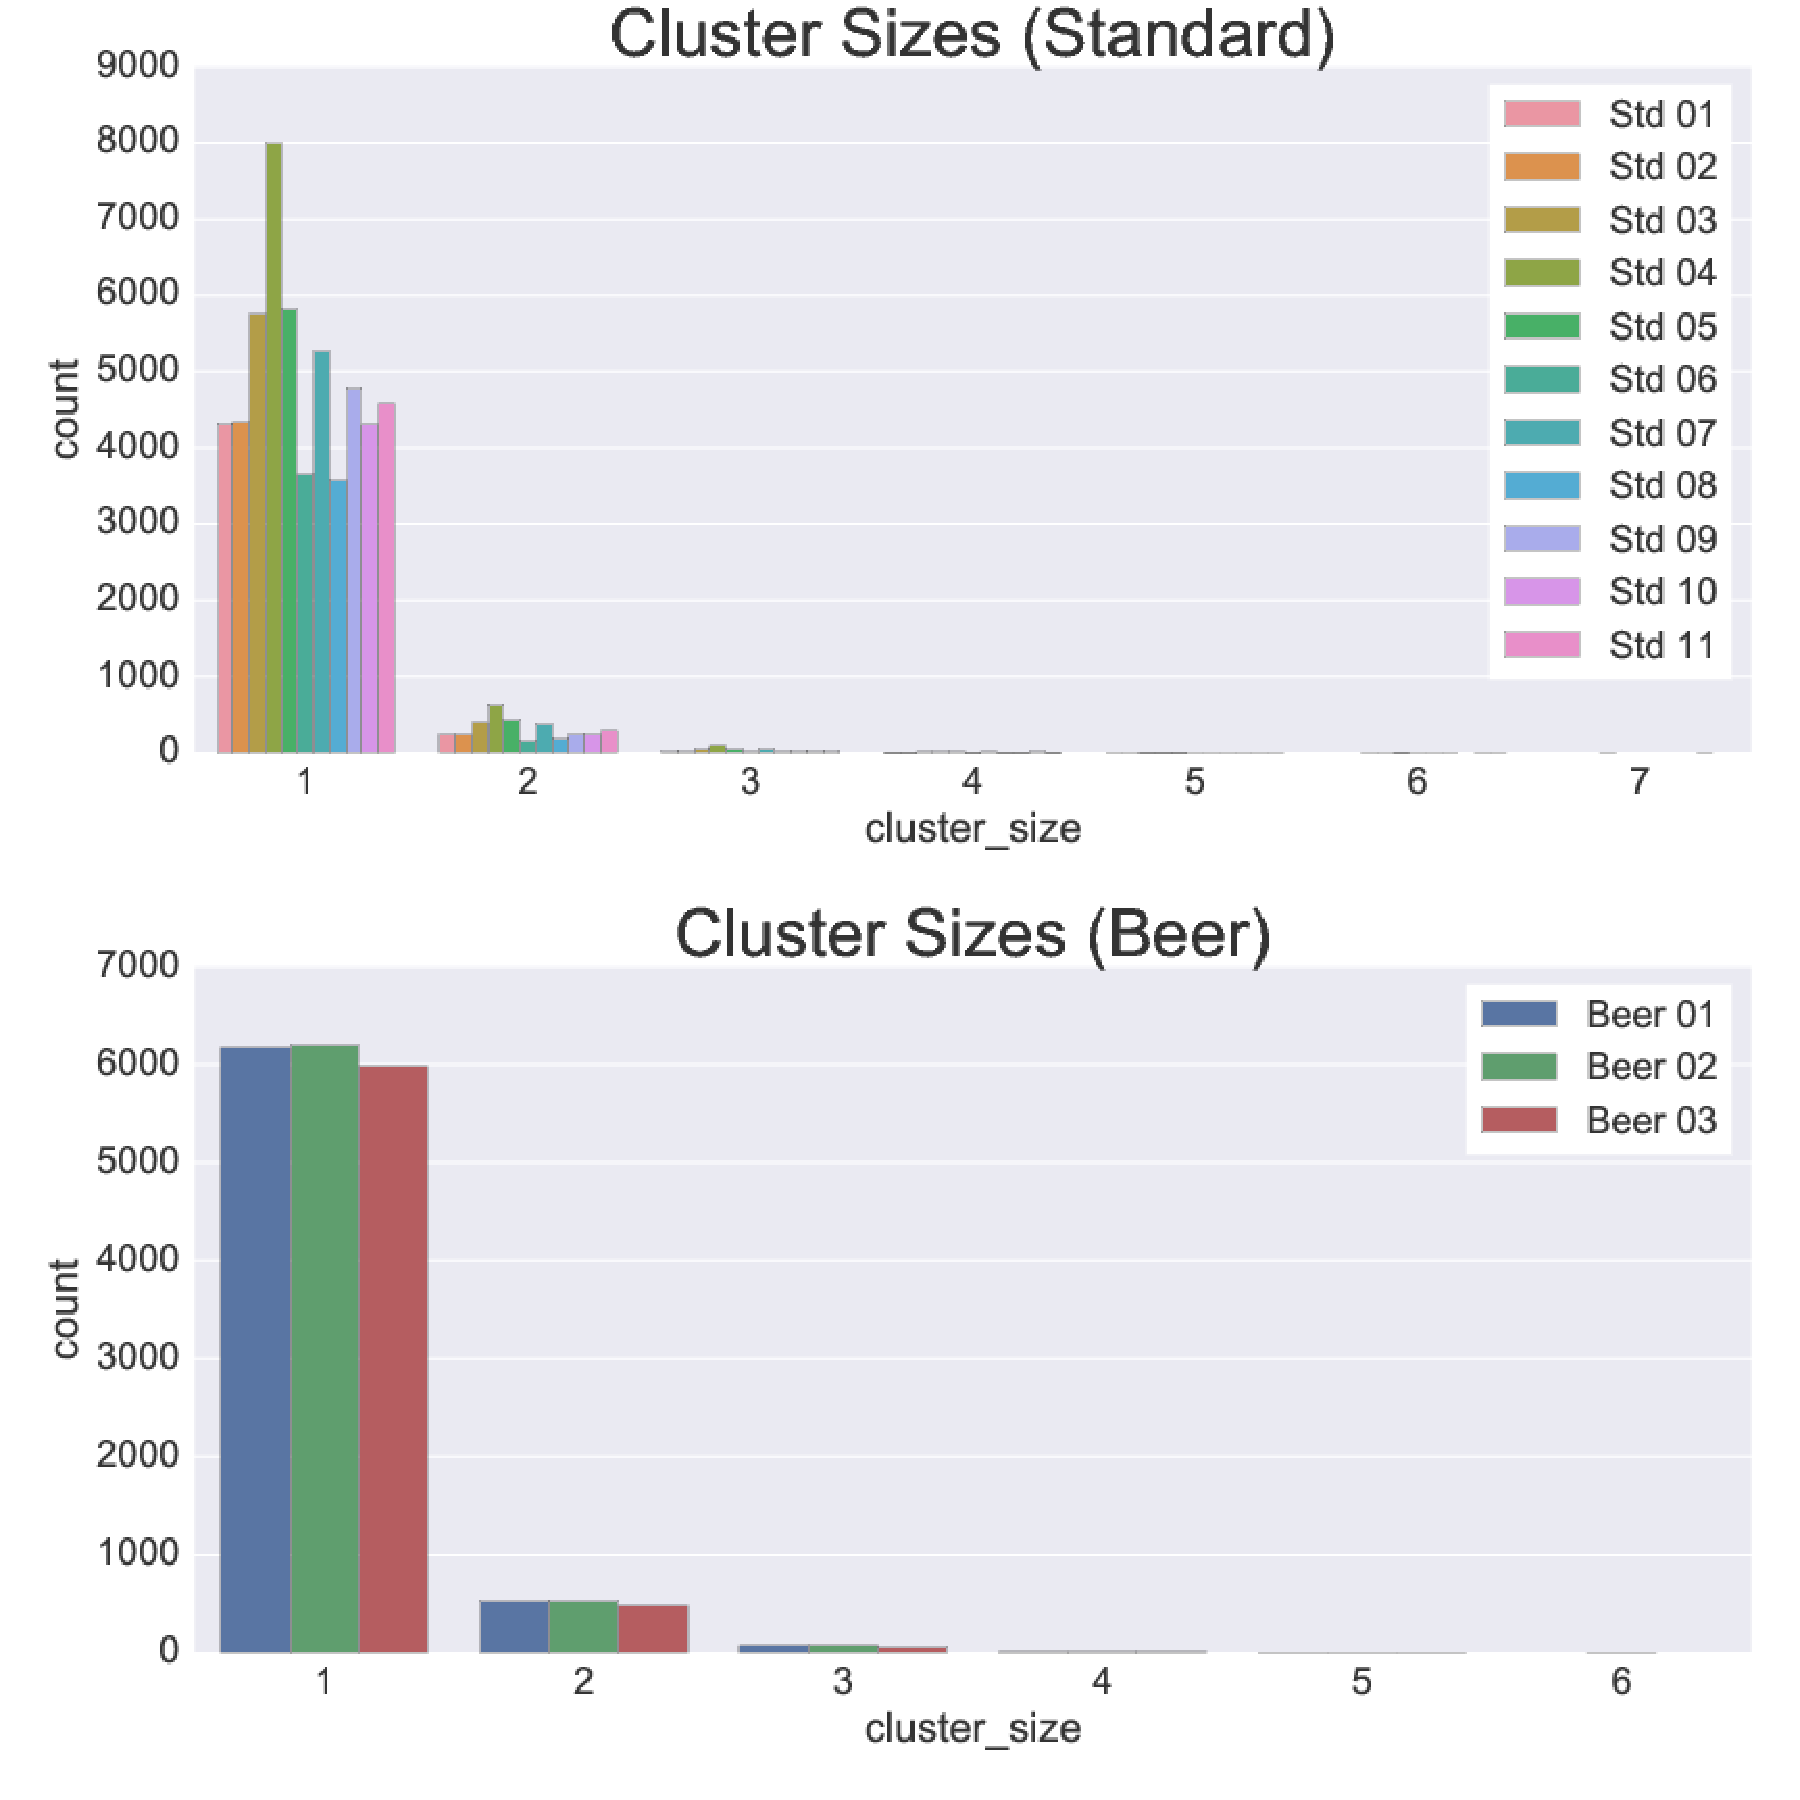
\includegraphics[width=1.0\linewidth]{05-precursor-cluster/figures/counts_cluster.pdf}
\caption{\label{fig:cluster-counts} Ionization product cluster sizes for all runs in the Standard and Beer datasets. For any given size, the number of clusters are generally more consistent in the Beer runs compared to the Standard runs, which shows greater variability due to the differences in the number of peak features per run.}
\end{figure}

%\begin{table}
%\centering
%\caption{The number of peak features and the counts of singleton and non-singleton IP clusters in each run of the Standard and Beer datasets. A singleton cluster is defined to be an IP cluster having only one member peak after MAP assignments, while a non-singleton IP cluster has more than one member peaks. The last column in the Table shows the counts of non-singleton IP clusters and also the percentage of non-singleton IP clusters from the total IP clusters in that run. \label{Tab:cluster-counts}}
%\begin{tabular}{|c|c|c|>{\centering}p{0.1\textwidth}|}
%\hline 
%Data & \# Peak Features & \# Singleton IP Cluster & \# Non- singleton IP Cluster\tabularnewline
%\hline 
%\hline 
%Std 01 & 4999 & 4327 & 301 (6.5\%)\tabularnewline
%\hline 
%Std 02 & 4986 & 4341 & 288 (6.2\%)\tabularnewline
%\hline 
%Std 03 & 6836 & 5755 & 481 (7.7\%)\tabularnewline
%\hline 
%Std 04 & 9752 & 8011 & 775 (8.8\%)\tabularnewline
%\hline 
%Std 05 & 7076 & 5801 & 551 (8.7\%)\tabularnewline
%\hline 
%Std 06 & 4146 & 3655 & 216 (5.6\%)\tabularnewline
%\hline 
%Std 07 & 6319 & 5272 & 469 (8.2\%)\tabularnewline
%\hline 
%Std 08 & 4101 & 3579 & 232 (6.1\%)\tabularnewline
%\hline 
%Std 09 & 5485 & 4789 & 312 (6.1\%)\tabularnewline
%\hline 
%Std 10 & 5034 & 4304 & 310 (6.7\%)\tabularnewline
%\hline 
%Std 11 & 5317 & 4574 & 337 (6.8\%)\tabularnewline
%\hline 
%Beer 01  & 7553 & 6179 & 633 (9.3\%)\tabularnewline
%\hline 
%Beer 02 & 7579 & 6203 & 631 (9.2\%)\tabularnewline
%\hline 
%Beer 03 & 7240 & 5983 & 574 (8.6\%)\tabularnewline
%\hline 
%\end{tabular}
%\end{table}

It is also interesting to examine the MAP transformation types and the resulting probabilities on those transformation produced by PrecursorCluster on the Standard and Beer runs. Consistent with the number of singleton clusters, the M+H transformation dominate in the data. Non M+H transformations comprise only 8\% of the total MAP transformations for the Standard dataset and 10\% for the Beer dataset. Figures~\ref{fig:trans-standards}A and \ref{fig:trans-beer}A show the counts of transformation types inferred for each run in the Standard and Beer datasets after MAP assignments. We see that in the Standard runs, the M+Na and M+ACN+H transformation types are highly prevalent (Figure~\ref{fig:trans-standards}A), while in the Beer runs, M+ACN+H and M+CH3OH+H are among the top most-frequently observed transformation types ((Figure~\ref{fig:trans-beer}A). The presence of ACN clusters in the results are entirely expected, given the acetonitrile buffer used during HPLC.

From the boxplots of assignment probabilities in Figures~\ref{fig:trans-standards}B and \ref{fig:trans-beer}B, we also see that PrecursorCluster is generally confident (with most probabilities approaching 1.0) in its MAP assignments of peaks to IP clusters through the adduct transformation types listed in Table~\ref{Tab:transformation}. In particular, this applies to the most prevalent transformation types of M+Na and M+ACN+H in both the Standards and Beer datasets. We also see from the boxplots in Figure~\ref{fig:trans-standards}B and \ref{fig:trans-beer}B and that the transformation types having the largest interquartile range (M+2ACN+H in the Standard runs, M+ACN+Na in the Beer runs) are generally not the most prevalent ones in the dataset.

\begin{figure}[!htbp]
\centering
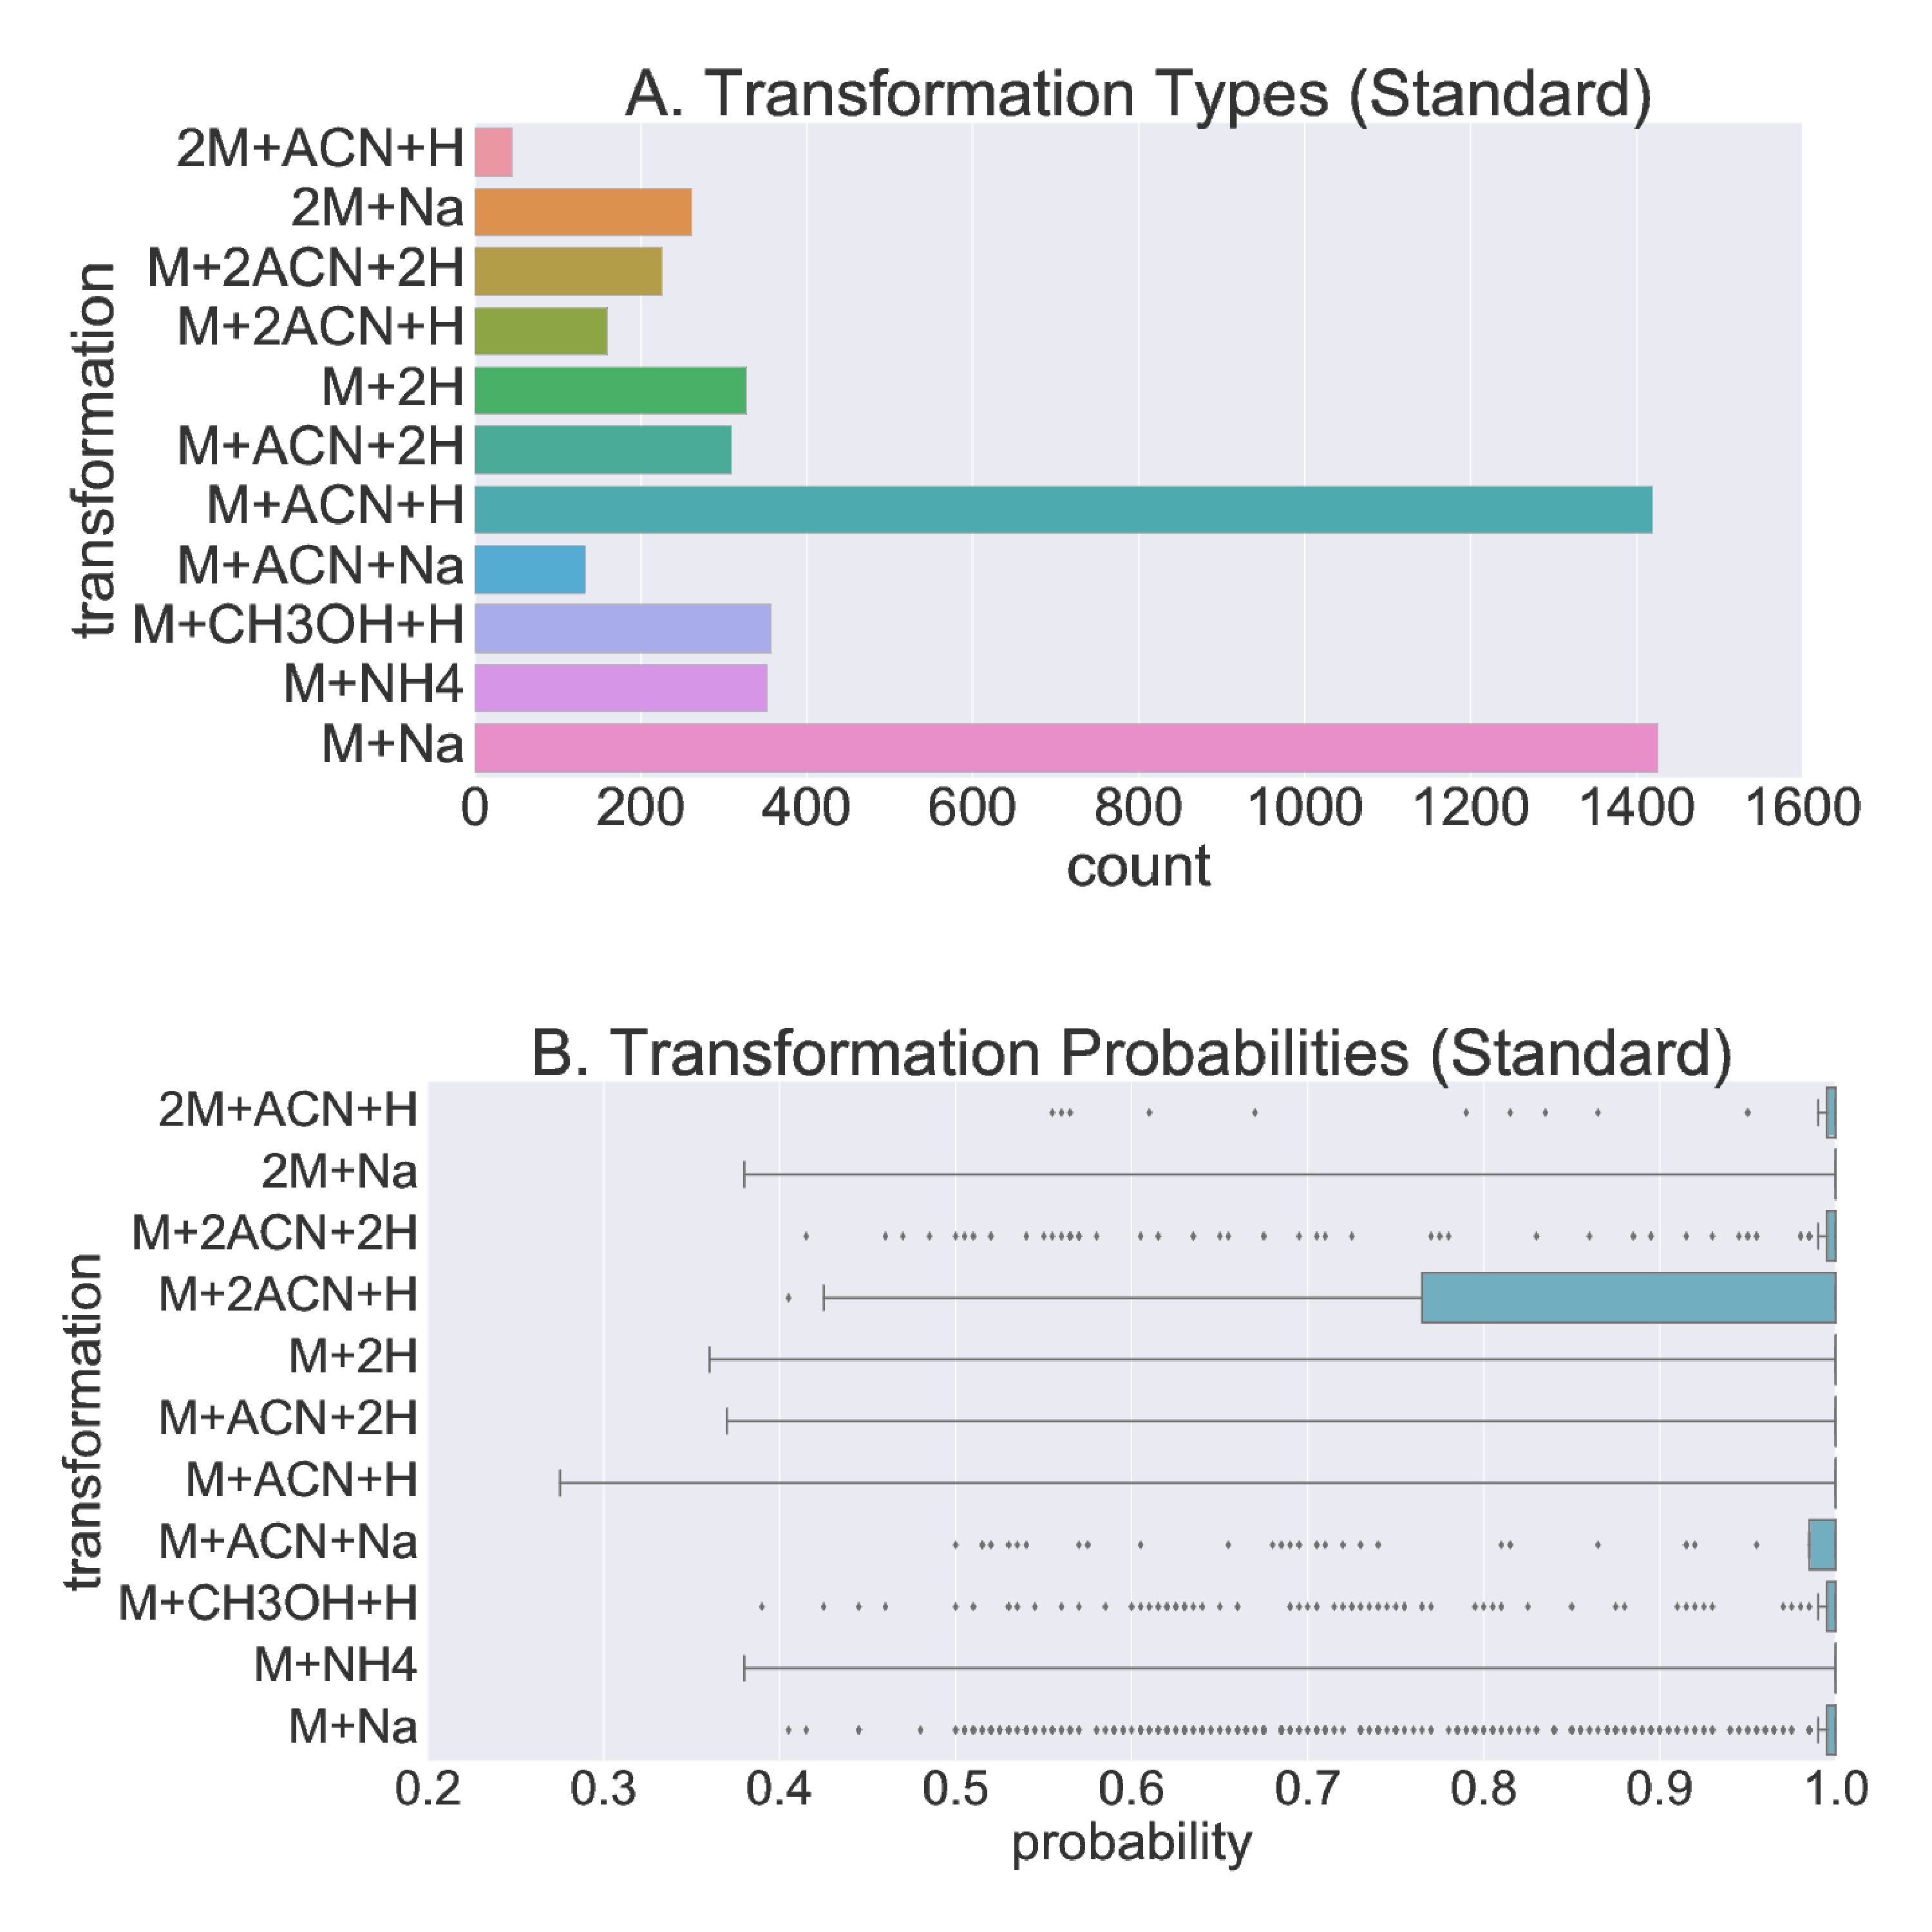
\includegraphics[width=1.0\linewidth]{05-precursor-cluster/figures/trans_Standard.pdf}
\caption{\label{fig:trans-standards} \textbf{(A)} Barcharts showing the counts of transformation types in each Standard run. We see that the top two most-occurring transformation types are M+Na and M+ACN+H. \textbf{(B)} Boxplots with confidence interval showing the probabilities of transformation types across all Standard runs. With the exception of M+2ACN+H, we observe high confidence in the assignment of peaks into an IP cluster through any of the listed transformation types.}
\end{figure}

\begin{figure}[!htbp]
\centering
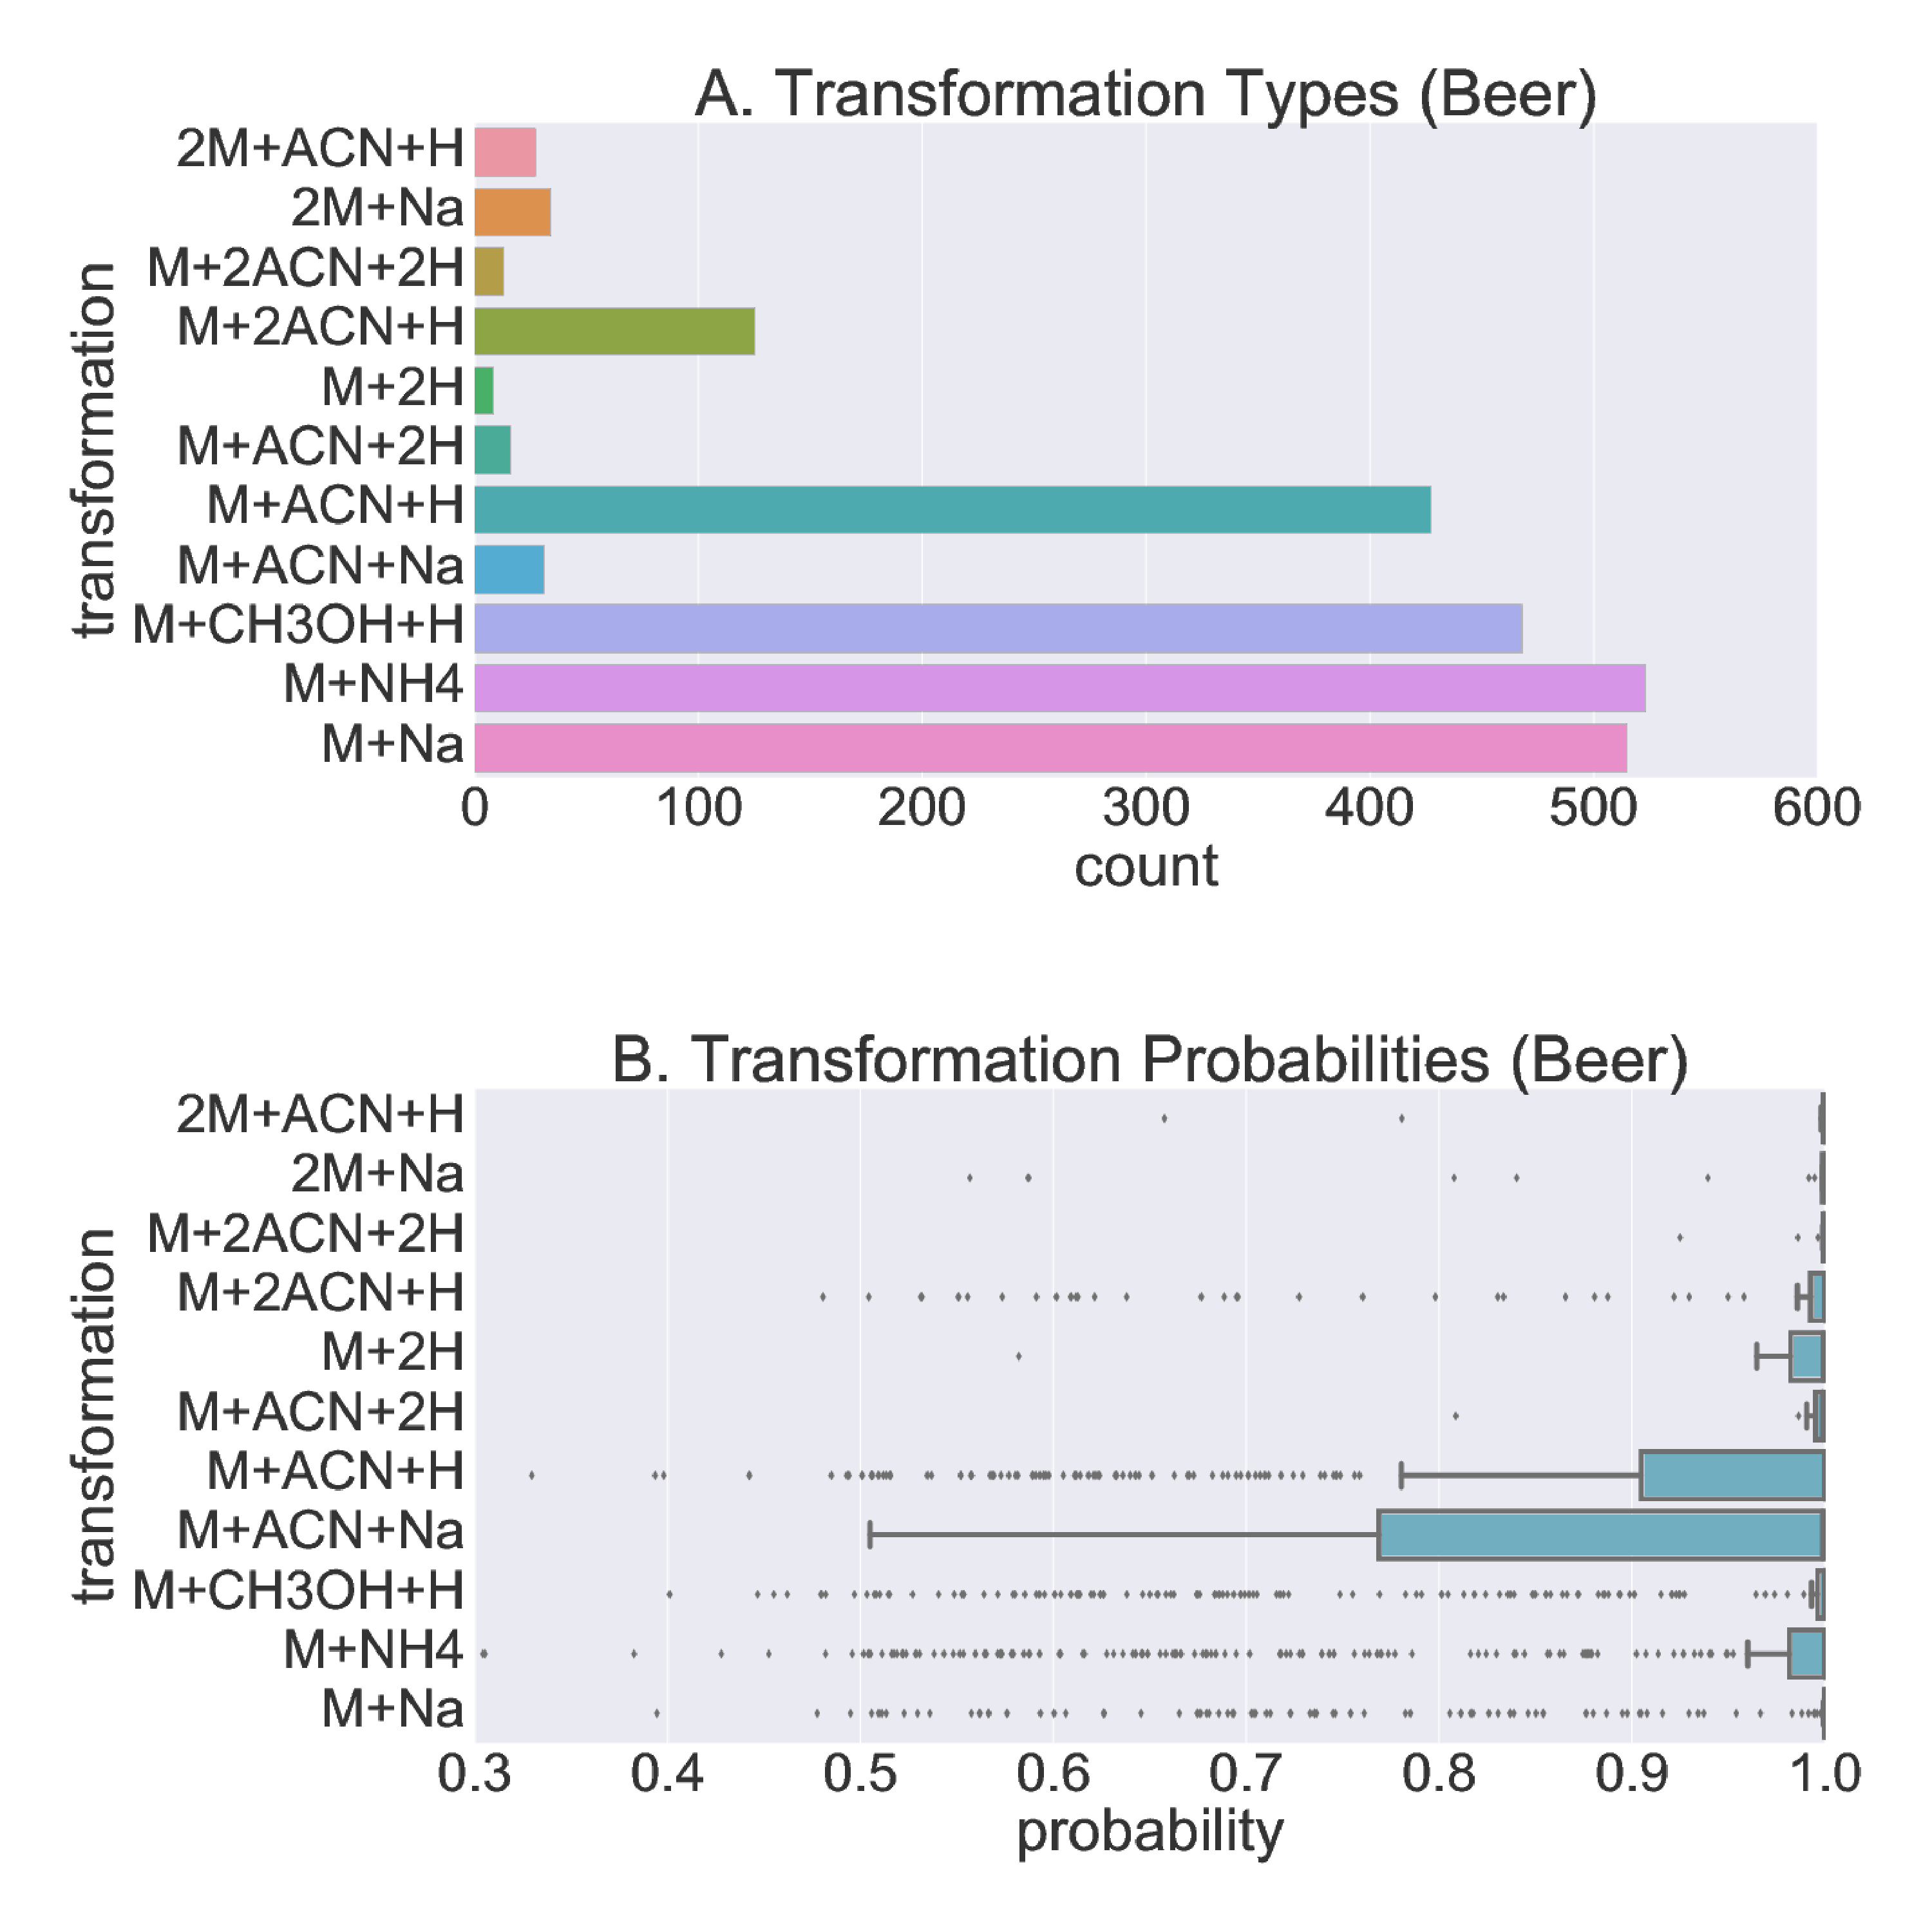
\includegraphics[width=1.0\linewidth]{05-precursor-cluster/figures/trans_Beer.pdf}
\caption{\label{fig:trans-beer} \textbf{(A)} Barcharts showing the counts of transformation types in each Beer run. We see that the top three most-occurring transformation types are M+Na, M+NH4 and M+CH3OH+H. \textbf{(B)} Boxplots with confidence interval showing the probabilities of transformation types across all Beer runs. With the exception of M+ACN+H and M+ACN+Na, we observe high confidence in the assignment of peaks into an IP cluster through any of the listed transformation types.}
\end{figure}

A complete investigation on how the ionization prevalence of metabolites present in the two datasets differs is beyond the scope of this paper. Notably, our PrecursorCluster model can easily take into account the ionization product clustering of LC-MS peak features based on isotope transformations (e.g. C$_{13}$) as well. Running PrecursorCluster by taking into account the adduct transformation types alongside the C$_{13}$-isotope transformation type shows that twice as many non-singletons can be obtained per run (see Supplementary \textbf{S.XXX} for details). However, as Figure~\ref{fig:more-uncertainty} shows with the Beer data as an example, this increase in the number of non-singleton clusters is also accompanied by an increase in assignment uncertainties of LC-MS peak features into any given IP cluster. Since in our current workflow, each run is modelled independently, incorporating isotope rule into PrecursorCluster makes establishing a consistent MAP assignment (for the purpose of aligning IP clusters across runs) difficult. As such, for subsequent alignment results in Section~\ref{sub:cluster-match-results} and \ref{sub:cluster-cluster-results}, we use only the results from running PrecursorCluster with the adduct transformation rules only. While it is beyond the scope of this paper, taking isotope transformation into consideration appears to be necessary if we were to consider using the results from PrecursorCluster differently, e.g. for the putative annotations of metabolites, and is an avenue worth investigating in detail.

\begin{figure}[!htbp]
\centering
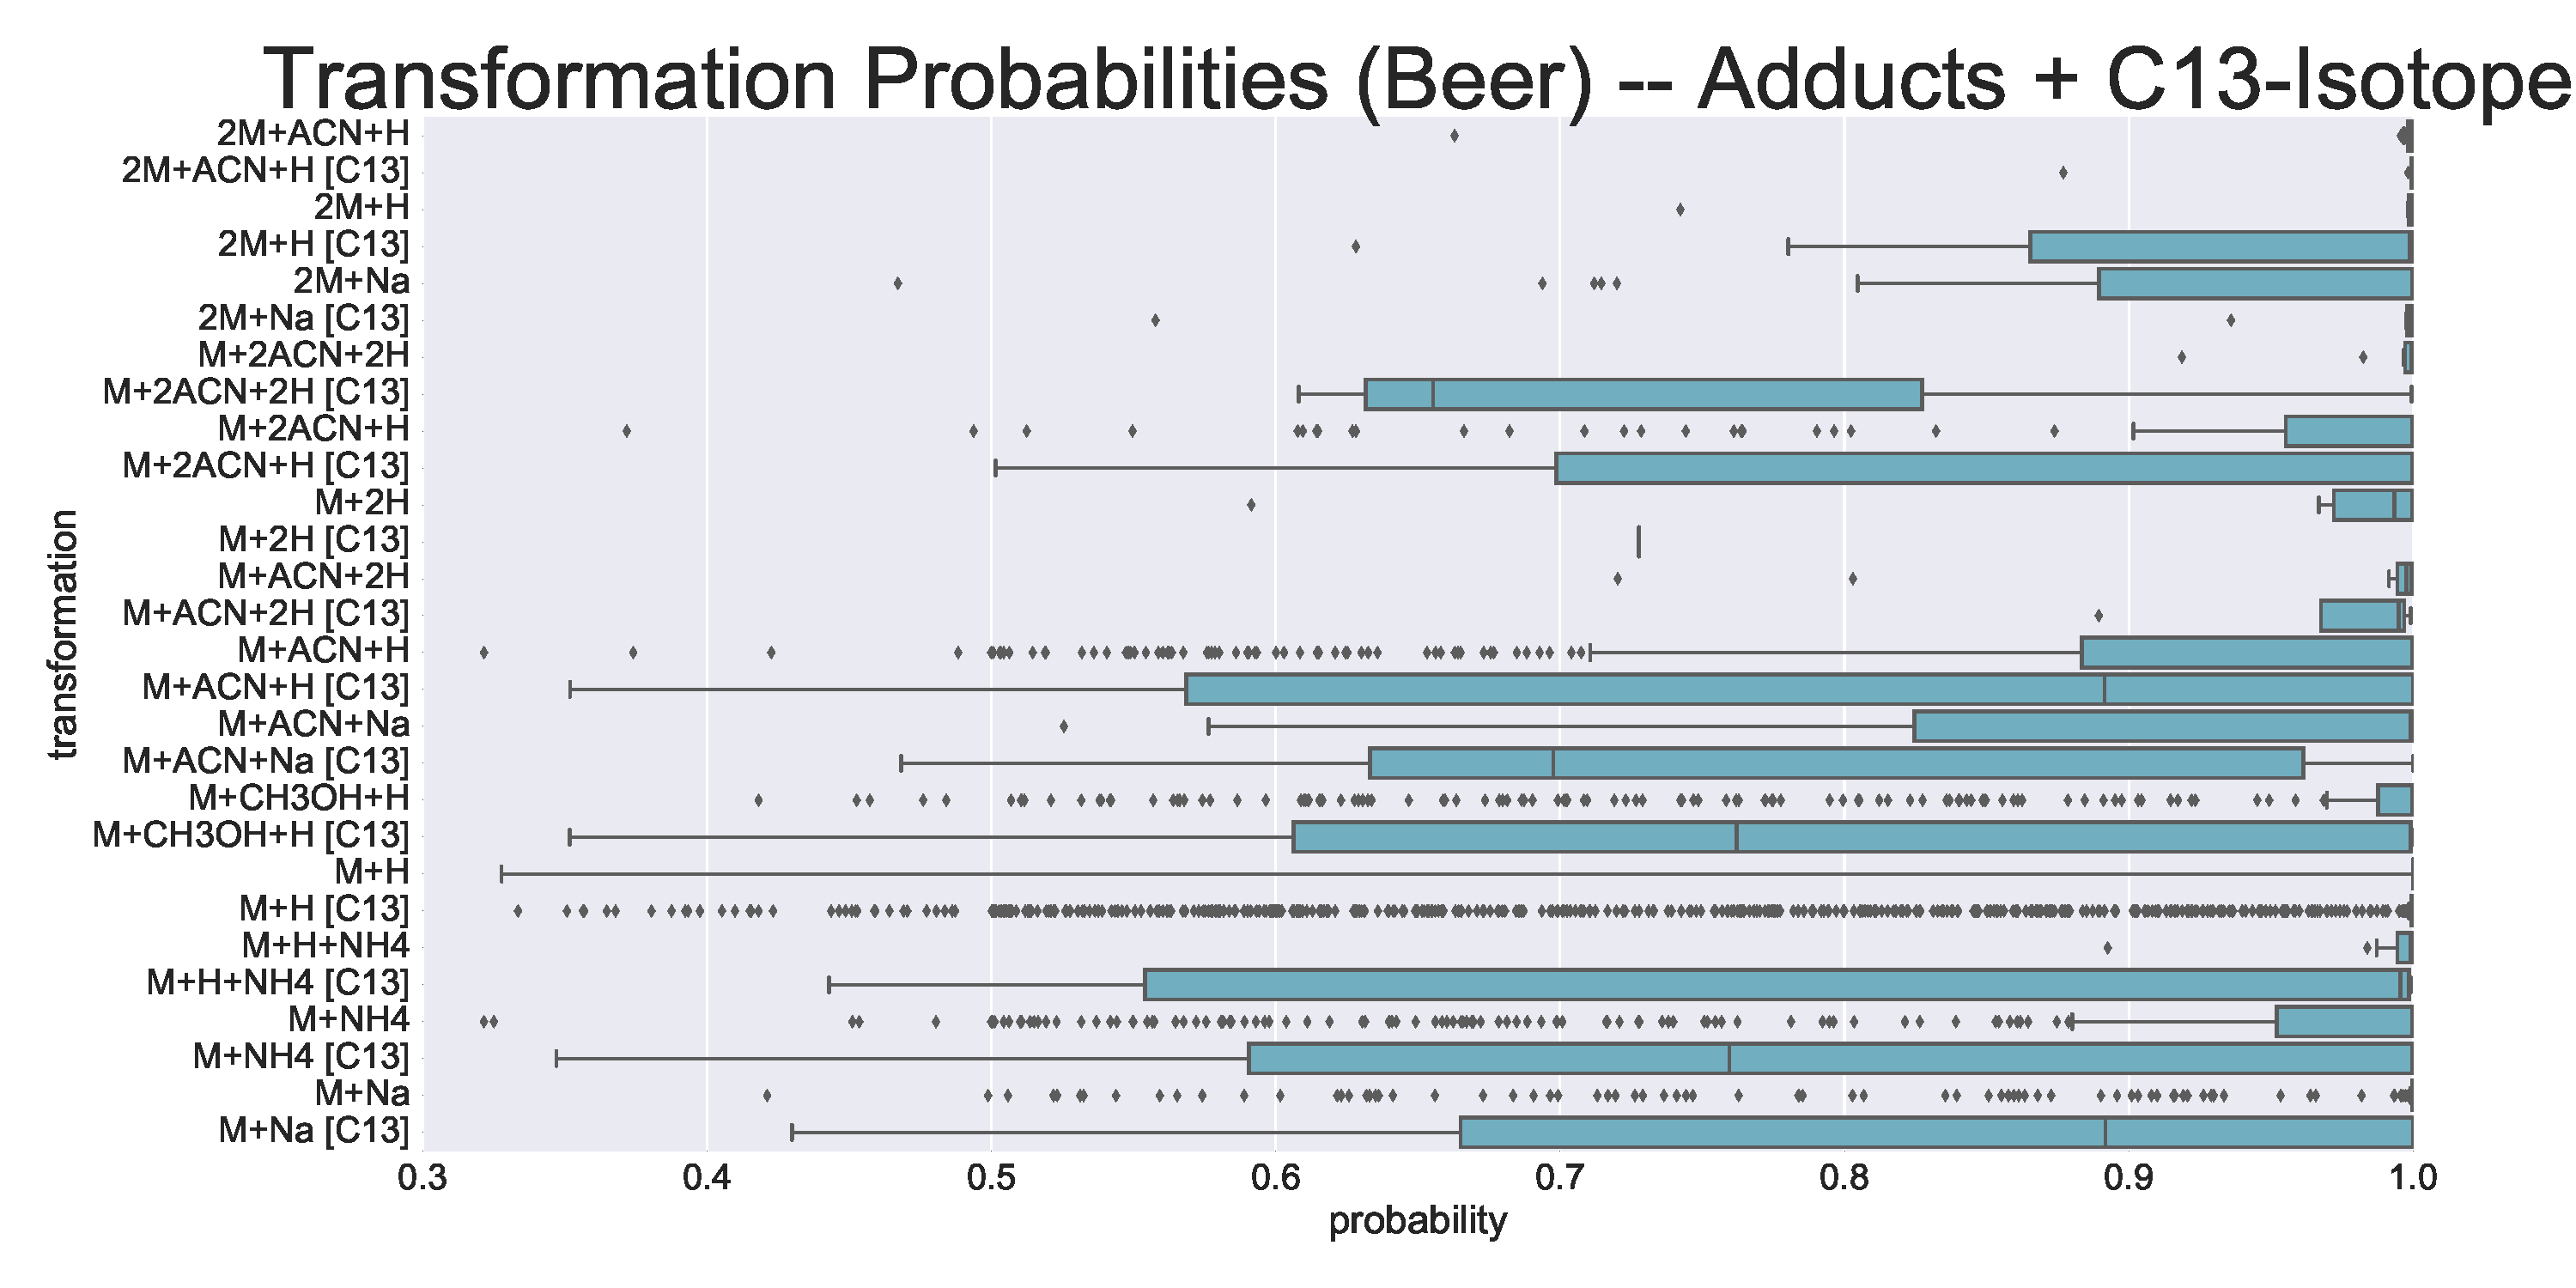
\includegraphics[width=1.0\linewidth]{05-precursor-cluster/figures/prob_trans_Beer_2.pdf}
\caption{\label{fig:more-uncertainty} Boxplots with confidence interval showing the probabilities of transformation types across all Standard runs when both the adduct transformation types (Table~\ref{Tab:transformation}) and the C$_{13}$-isotope transformation type are used. The increase in assignment uncertainties compared to Figure~\ref{fig:trans-beer}B makes it difficult to establish consistent MAP-assignment of peak features into the same IP clusters across runs. }
\end{figure}

\subsection{Improved peak alignment performance by using clustering information in Cluster-Match}

Figure~\ref{fig:training-results} shows the density plots of all the training precision and recall values produced by the different methods from the entire 30 training sets of pairwise Standard runs and the 3 Beer runs. Here, we set $l$ (the size of peakset combinations to be considered during performance evaluation) to 2 to consider only pairwise features for performance evaluation. The results in Figure~\ref{fig:training-results} (top row) shows that across all the m/z and RT window tolerances varied, Cluster-Match can produce higher precision while retaining similar recall values to feature matching (MW) or modified feature matching (MWG). This increase in precision comes from the increase of true positives and the decrease in false positives by taking into account the ionization product relationships between peak features when constructing the matching. The results here suggest that, regardless of the parameters selected for the m/z and RT tolerance windows, the proposed methods of matching by IP clusters can return a better alignment result (as measured by precision and recall) compared to matching by peak features only.

Similar results can also be observed for the Beer dataset (Figure~\ref{fig:training-results}, bottom row). The complex Beer runs being aligned have minimal RT deviations when compared to the Standard runs, so all evaluated methods perform well, demonstrating smaller deviations in performance values despite varying the tolerances parameters. Again here we see a general increase in precision of the results from Cluster-Match over the other two baseline methods. The MWG method, which relies on the grouping of related peaks using their retention time values only, does not appear to produce any improvements over MW. The results here suggest that on complex LC-MS data such as the Beer data, the richer information present in the m/z and RT values of related peak features, alongside their possible IP transformations and relationships to the precursor peak, is essential and has to be taken into account.

\begin{figure*}[!htbp]
\centering
\centering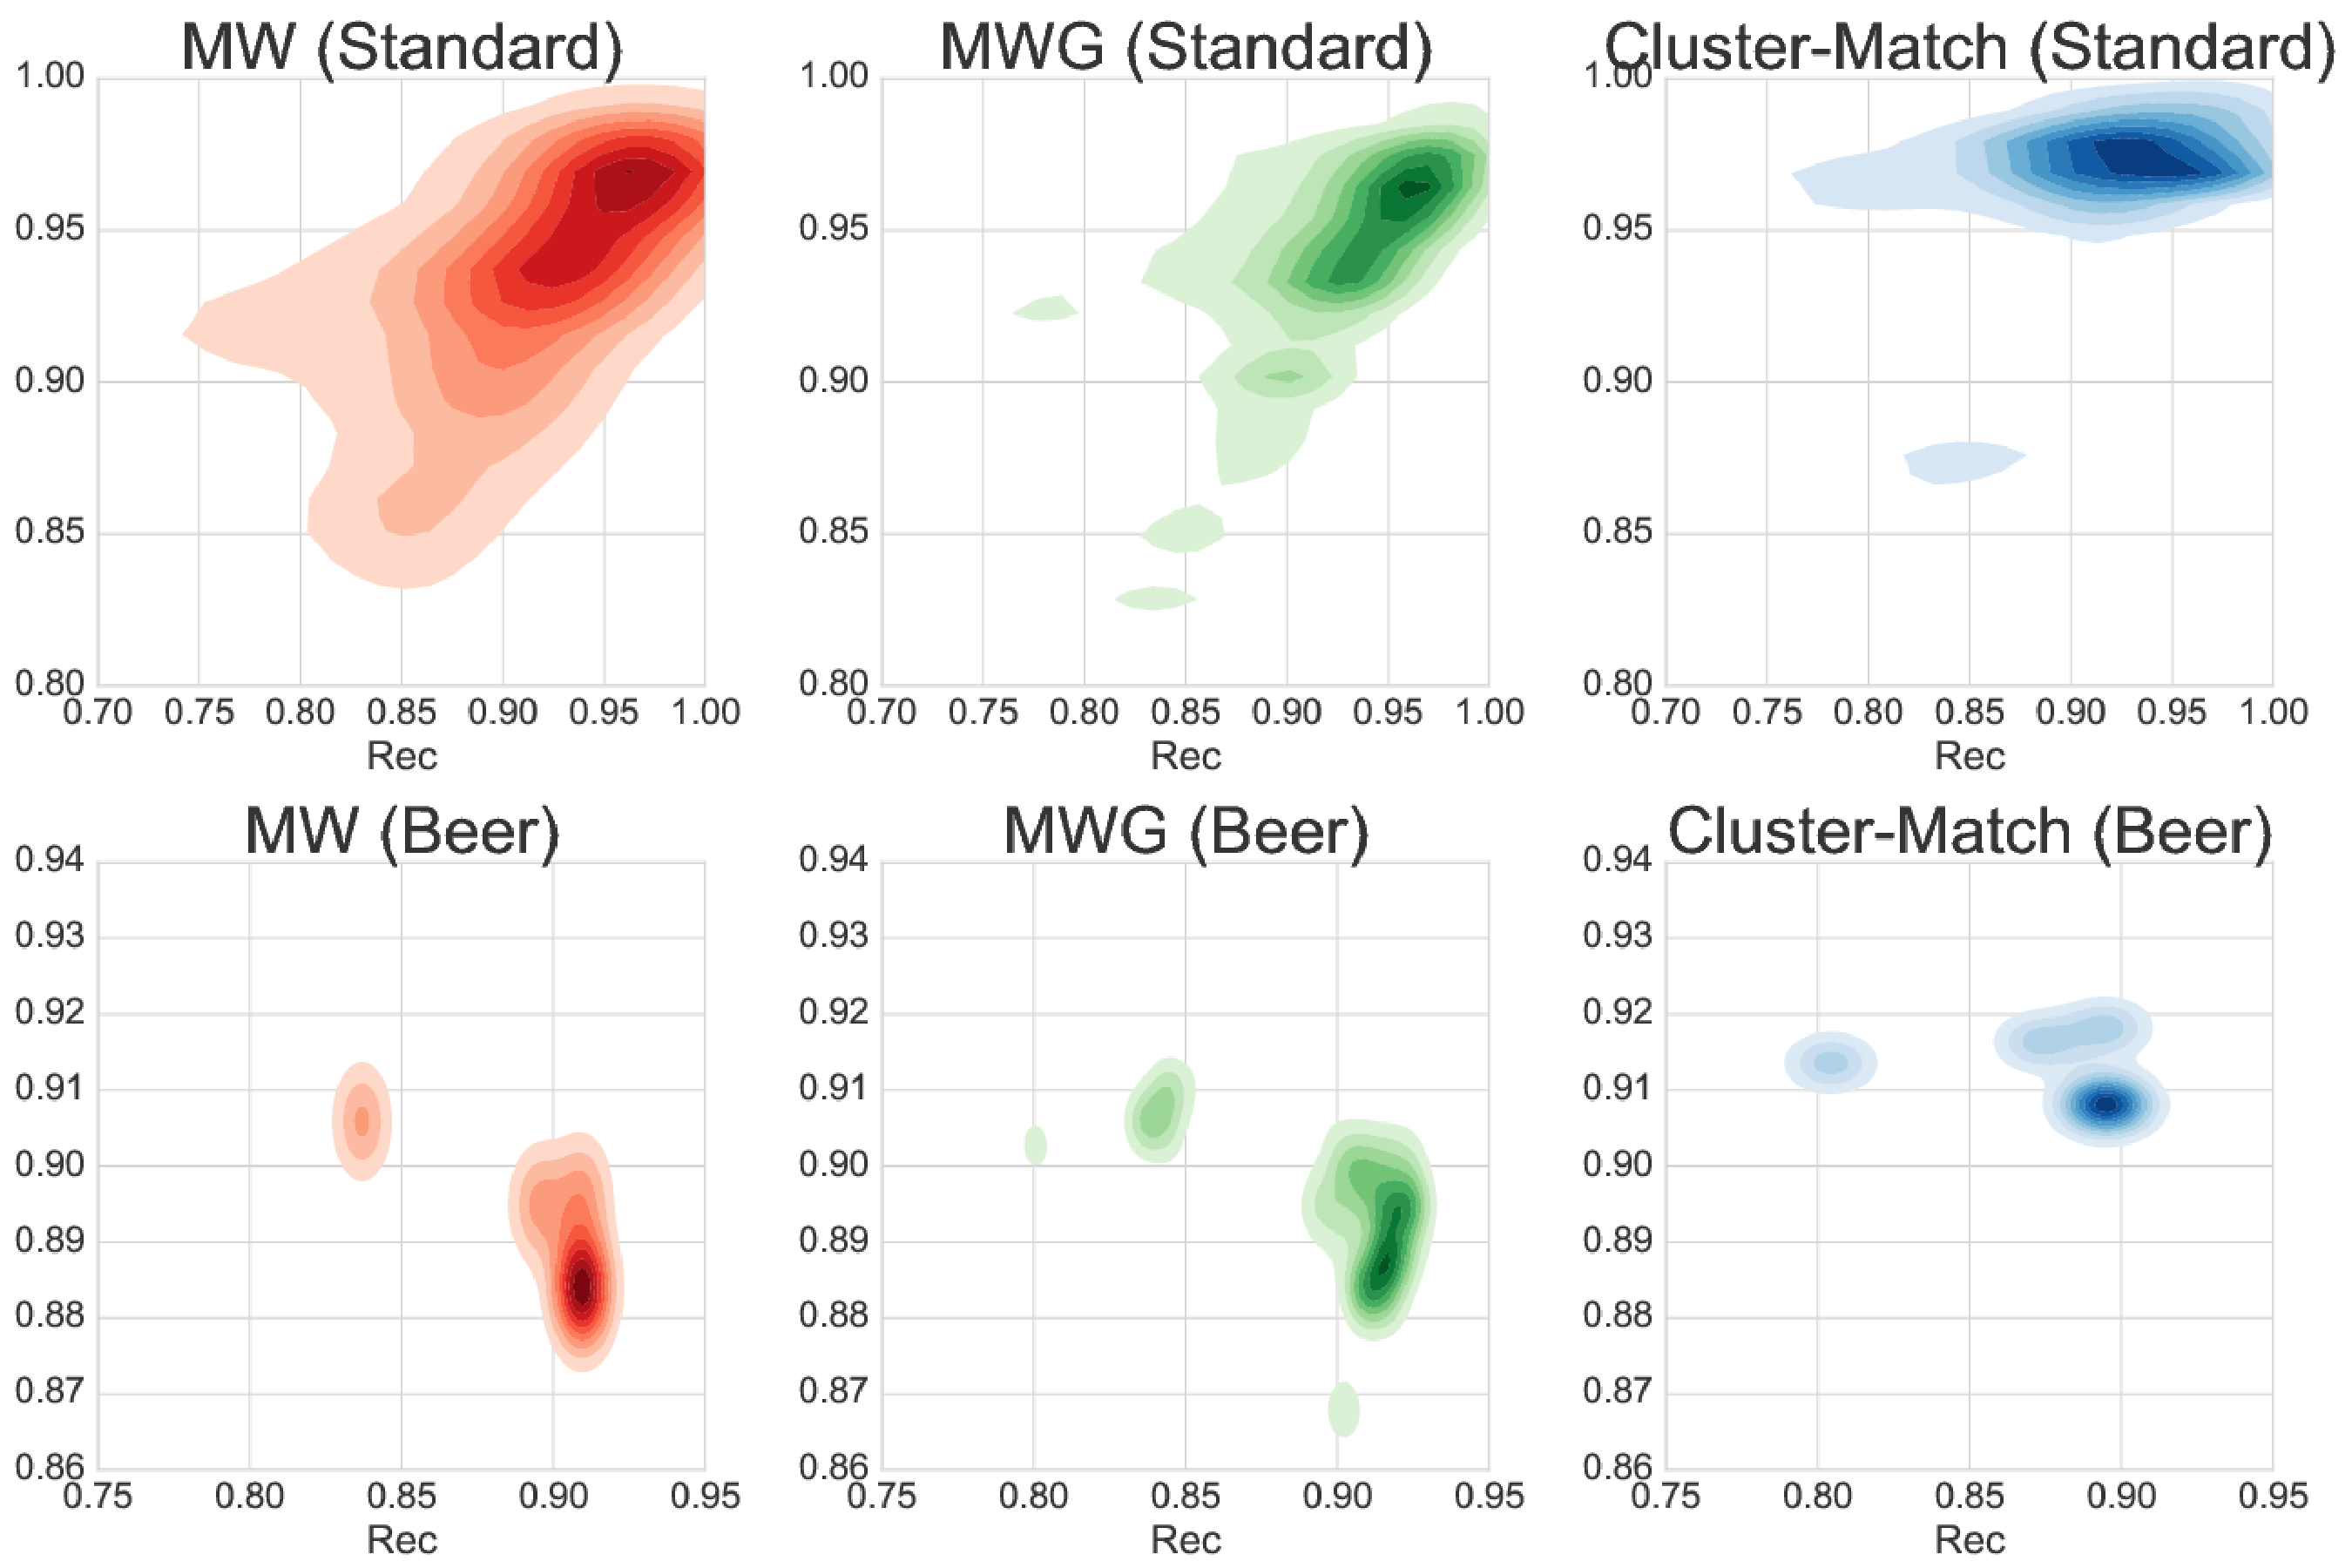
\includegraphics[width=1.0\linewidth]{05-precursor-cluster/figures/fig2.pdf}
\caption{\label{fig:training-results} All the training results obtained by varying the m/z and RT window parameters from the alignment of the entire 30 sets of pairwise Standard runs (top row) and the 3 Beer runs (bottom row). For MWG, the grouping parameter $t$ and score contribution $\alpha$ were also varied, while for Cluster-Match, the same set parameters of first-stage clustering was used for all input files.}
\end{figure*}

The next results of Figure~\ref{fig:pairwise-training-testing} combine precision and recall into a single measure of $F_1$-score and evaluate how the different alignment methods evaluated might generalize to new and unseen datasets. In Figures~\ref{fig:pairwise-training-testing}, we report the best $F_1$-scores produced by each method on the 30 sets of training and testing Standard runs. Consistent with the improvements in precision from the training results, the results here show that Cluster-Match is able to produce higher training and testing $F_1$-scores compared to MW. Using a one-sided paired t-test, the means of the $F_1$-scores for MW are found to be statistically less than that of Cluster-Match in both the training (p-value=0.002) and the testing cases (p-value=0.026). On the training results, MWG produces even higher training $F_1$-scores compared to the other two methods methods. This difference is found to be statistically significant using a one-sided paired t-test (p-value=0.01). The higher training performance of MWG can be explained by the fact that the RT grouping tolerance parameter $t_g$ and matching ratio $\alpha_g$ for MWG were also optimized for each training set during the training phase, whereas the same set of clustering parameters were used when performing the first-stage clustering for each run in the PrecursorCluster model. On the testing results, we found no statistically significant differences on the testing $F_1$-scores of MWG and Cluster-Match, suggesting that both methods generalize well to new and unseen data. Taken together, our results demonstrate that in general, constructing alignment by working with groups of related peaks (Cluster-Match) results in a better alignment performance compared to alignment based on individual peak features (MW).

\begin{figure}[!htbp]
\centering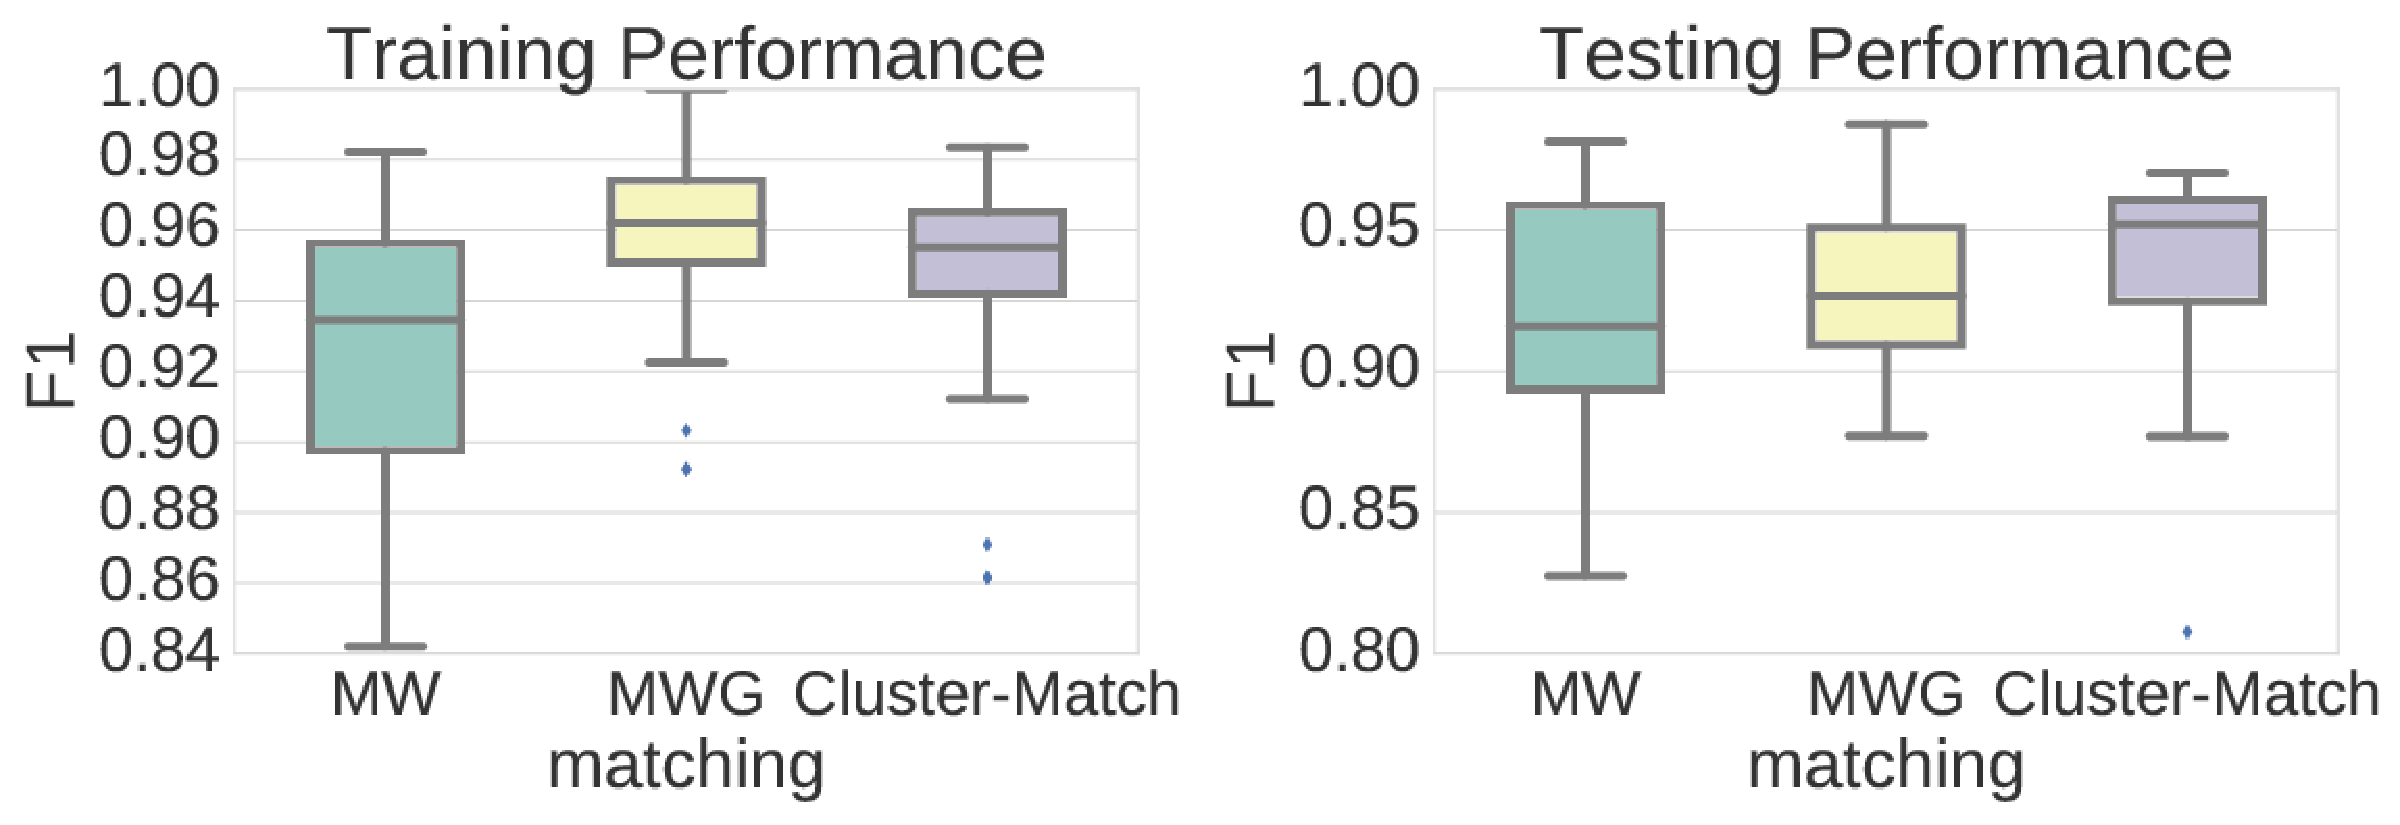
\includegraphics[width=1.0\linewidth]{05-precursor-cluster/figures/fig3.pdf}
\caption{\label{fig:pairwise-training-testing} The best training and testing $F_1$-scores obtained from the alignment of 30 sets of Standard runs.}
\end{figure}

% The results here suggest on that the best training parameters (in particular, the $t_g$ and $\alpha_g$ parameters) for MWG do not generalise as well as Cluster-Match, where the same set of parameters were used throughout the first-stage precursor clustering, when applied onto the testing datasets. The best within-file grouping tolerance from the training stage relies on the RT information of peak features only. This does not generalize across runs as well as the first-stage ionization product clustering used for Cluster-Match, which takes into account the richer information present in the m/z and RT values of related peak features alongside their possible ionization product transformations and relationships to the precursor peak. 

\subsection{Probabilistic matching results from Cluster-Cluster}

Direct-matching methods such as MW and Cluster-Match can only return a definite matching solution to the alignment problem (a peak from one run is either aligned to a peak in the other run, or not). In contrast, the second-stage clustering process of the IP clusters employed in the Cluster-Cluster method allows us to produce an estimate in the uncertainties of matching of peak features, producing as the alignment result a list of aligned peaksets that have been matched at varying levels of confidence. Figure~\ref{fig:pr-curve} shows how a Precision-Recall (PR) curve, which shows how precision and recall change together, can be computed from the output of Cluster-Cluster on one of the sets of 4 randomly selected Standard runs and the set of 3 Beer runs. In Figure~\ref{fig:pr-curve}, the PR curves are plotted alongside the results from Cluster-Match at varying m/z and RT tolerance parameters (note that for Cluster-Cluster, we used only one set of potentially sub-optimal parameters for the second-stage clustering). Along both the PR curves on Figure~\ref{fig:pr-curve}, we see that generally, a decrease in the recall values is accompanied by an increase in the precision values. This applies to both the Standard and the Beer datasets, suggesting that by setting an appropriate threshold on the probabilities of aligned peaksets returned by Cluster-Cluster, we can obtain fewer aligned peaksets (lower recall) but at a higher confidence level of being correctly aligned (higher precision).

In the face of further uncertainties with regard of user-defined parameters from the previous parts of the pipeline, the probabilistic alignment results returned by Cluster-Cluster allows the user to focus on peaksets of high matching confidence for subsequent analysis.  This introduces the possibility of returning a smaller subset from the overall aligned peaksets that have a higher confidence score of being correctly aligned -- an ability that few other matching methods can provide.

\begin{figure}[!htbp]
\centering
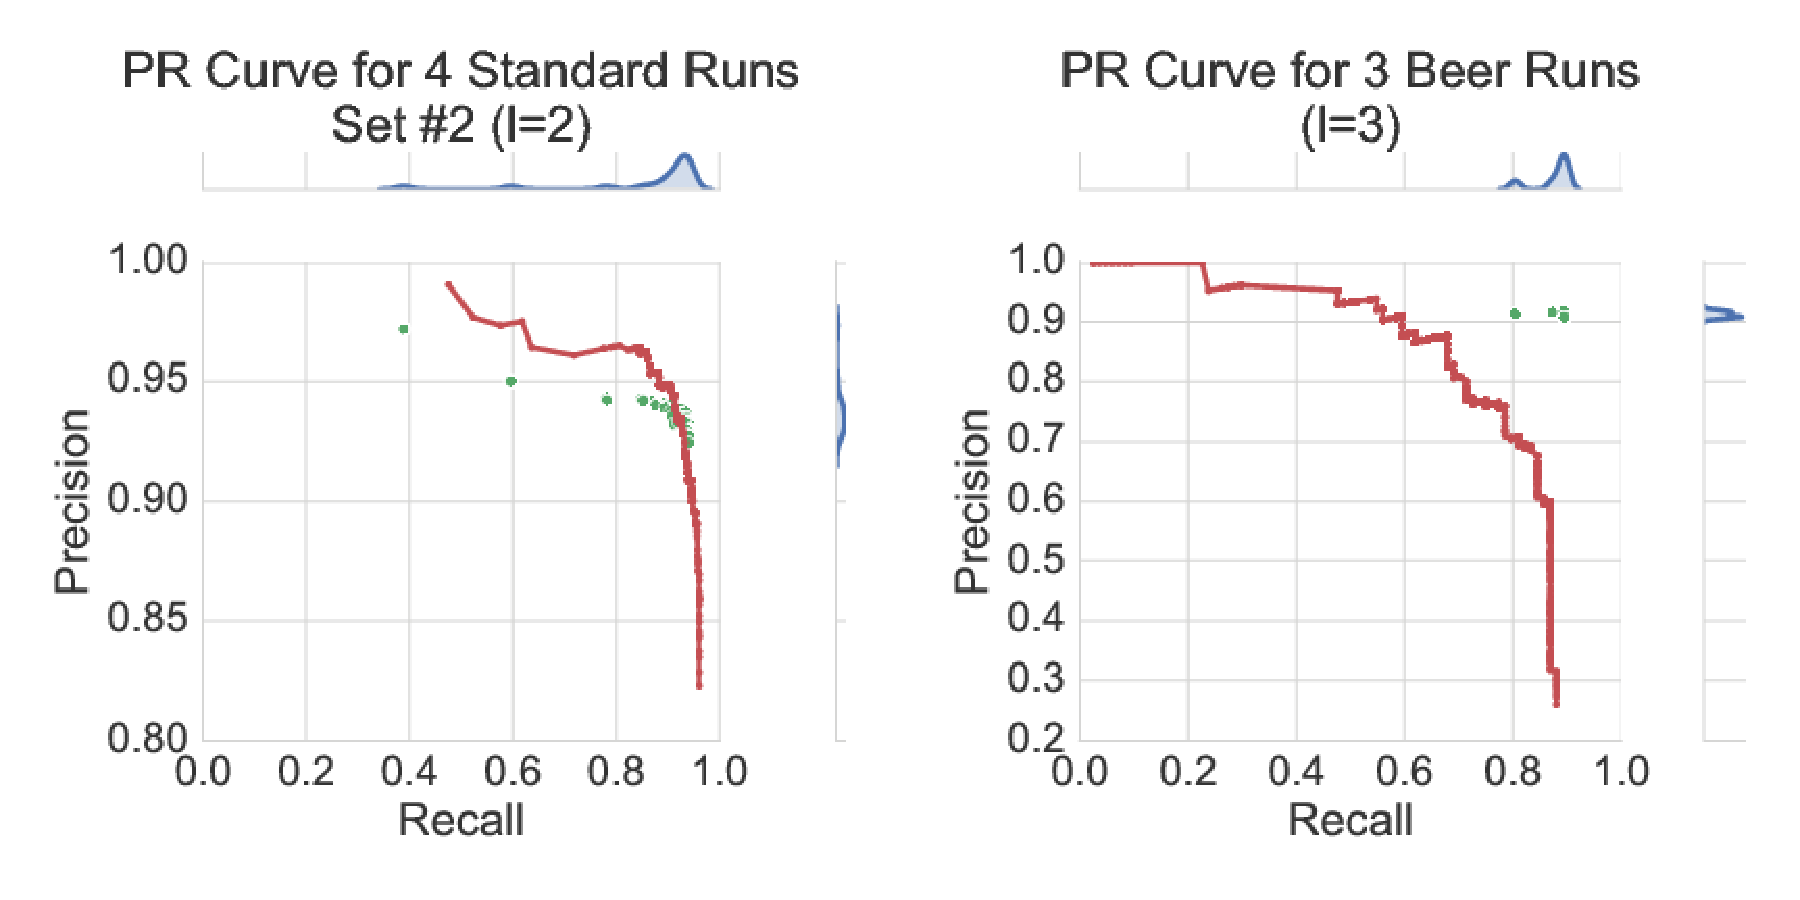
\includegraphics[width=1.0\linewidth]{05-precursor-cluster/figures/fig4.pdf}
\caption{\label{fig:pr-curve} PR curves obtained from running Cluster-Cluster on one of the sets of 4 randomly selected Standard runs (left) and the 3 Beer runs (right). Green dots are performance points obtained from running Cluster-Match at varying m/z and RT tolerance parameters on the same datasets, with their distributions of the points plotted along the marginals. The same first-stage clustering results were used as input to both Cluster-Match and Cluster-Cluster.}
\end{figure}

Indeed, the results from our experiments for Cluster-Cluster on the randomly selected sets of 2, 3, and 4 Standard runs (Table~\ref{Tab:standard-results}) and also on the 3 Beer runs (Table~\ref{Tab:beer-results}) show that by setting some threshold values $\{0.30, 0.60, 0.90\}$ on the probabilities of the alignment results returned by Cluster-Cluster, we can vary the resulting precision and recall values. For instance, when looking at the the alignment of 5 sets of four Standard runs in Table~\ref{Tab:standard-results} evaluated at strictness level $l=4$, we see that the best average performance from Cluster-Match is found at precision=0.87 and recall=0.92. At threshold=0.30, the result from Cluster-Cluster has a lower precision of 0.81 compared to Cluster-Match. By raising the threshold to 0.90 (consequently, decreasing recall as fewer aligned peaksets are now returned), we obtain from Cluster-Cluster an alignment result that has a higher precision value of 0.90. Results on the more complex Beer data (Table~\ref{Tab:beer-results}) also demonstrates the same point. Cluster-Cluster gives a precision value of 0.76 at threshold 0.30, which increases to 0.94 at threshold 0.90. Together, the results in Tables~\ref{Tab:standard-results} and ~\ref{Tab:beer-results}demonstrate that it is possible to extract subsets of the entire alignment results from Cluster-Cluster having a higher precision than can be attained by Cluster-Match with optimal m/z and RT tolerance values. Using Cluster-Cluster, the user can trade recall for precision; a potentially useful ability in the case where alignment ground truth is difficult to create or might not be available altogether, which is always the case in novel experiments. In this situation, it might make sense to focus analysis effort on aligned peaksets with high confidence values in which we can be more certain that they have been correctly aligned.

%\begin{table*}[!htbp]
%\centering
%\caption{Average precision, recall and $F_{1}$ values from Cluster-Cluster for randomly selected sets of 2, 3 and 4 Standard runs at varying strictness of evaluation ($l$) and thresholding levels $th=\{0.30, 0.60, 0.90\}$. The average performance is computed by averaging over the randomly selected 5 sets for each number of run. The best results from Cluster-Match and the result from running Cluster-Cluster without the adduct fingerprint term in the likelihood are also shown here for comparison. Note that for Cluster-Cluster, the results come from using one set of potentially sub-optimal parameters for the second-stage clustering.\label{Tab:standard-results}}
%\begin{tabular}{|l|c|c|c|c|>{\centering}p{0.1\textwidth}|>{\centering}p{0.1\textwidth}|>{\centering}p{0.1\textwidth}|>{\centering}p{0.1\textwidth}|>{\centering}p{0.1\textwidth}|}
%\hline 
%\multirow{2}{*}{Dataset} & \multirow{2}{*}{$l$} & \multicolumn{3}{c|}{Best Cluster-Match} & \multicolumn{4}{c|}{Cluster-Cluster} & Cluster-Cluster (without adduct term)\tabularnewline
%\cline{3-10} 
% &  & Avg. Prec. & Avg. Rec. & Avg. $F_{1}$ & Threshold & Avg. Prec. & Avg. Rec & Avg. $F_{1}$ & Avg. $F_{1}$\tabularnewline
%\hline 
%\hline 
%\multirow{3}{*}{Standard 2 runs} & \multirow{3}{*}{2} & \multirow{3}{*}{0.93} & \multirow{3}{*}{0.92} & \multirow{3}{*}{\textbf{0.93}} & 0.30 & 0.96 & 0.95 & 0.95 & \textbf{0.95}\tabularnewline
%\cline{6-10} 
% &  &  &  &  & 0.60 & 0.98 & 0.93 & \textbf{0.96} & 0.93\tabularnewline
%\cline{6-10} 
% &  &  &  &  & 0.90 & 1.00 & 0.90 & 0.94 & 0.80\tabularnewline
%\hline 
%\multirow{3}{*}{Standard 3 runs} & \multirow{3}{*}{3} & \multirow{3}{*}{0.89} & \multirow{3}{*}{0.90} & \multirow{3}{*}{\textbf{0.89}} & 0.30 & 0.82 & 0.91 & 0.84 & \textbf{0.86}\tabularnewline
%\cline{6-10} 
% &  &  &  &  & 0.60 & 0.86 & 0.88 & \textbf{0.86} & 0.85\tabularnewline
%\cline{6-10} 
% &  &  &  &  & 0.90 & 0.89 & 0.81 & 0.84 & 0.62\tabularnewline
%\hline 
%\multirow{3}{*}{Standard 4 runs} & \multirow{3}{*}{4} & \multirow{3}{*}{0.87} & \multirow{3}{*}{0.92} & \multirow{3}{*}{\textbf{0.89}} & 0.30 & 0.81 & 0.92 & 0.85 & \textbf{0.89}\tabularnewline
%\cline{6-10} 
% &  &  &  &  & 0.60 & 0.84 & 0.89 & 0.85 & 0.86\tabularnewline
%\cline{6-10} 
% &  &  &  &  & 0.90 & 0.90 & 0.83 & \textbf{0.86} & 0.65\tabularnewline
%\hline 
%\end{tabular}
%\end{table*}

% Preview source code from paragraph 36 to 37

%\begin{table*}[!htbp]
%\caption{Precision, recall and $F_{1}$ values from Cluster-Cluster for the 3 Beer runs at varying strictness of evaluation ($l$) and thresholding levels $th=\{0.30, 0.60, 0.90\}$. The best results from Cluster-Match and the results from running Cluster-Cluster without the adduct fingerprint term are also shown here for comparisons. Note that for Cluster-Cluster, the results come from using one set of potentially sub-optimal parameters for the second-stage clustering.\label{Tab:beer-results}}
%% Preview source code from paragraph 36 to 37
%\centering
%\begin{tabular}{|l|c|c|c|c|>{\centering}p{0.1\textwidth}|>{\centering}p{0.1\textwidth}|>{\centering}p{0.1\textwidth}|>{\centering}p{0.1\textwidth}|>{\centering}p{0.1\textwidth}|}
%\hline 
%\multirow{2}{*}{Dataset} & \multirow{2}{*}{$l$} & \multicolumn{3}{c|}{Cluster-Match} & \multicolumn{4}{c|}{Cluster-Cluster} & Cluster-Cluster (without adduct term)\tabularnewline
%\cline{3-10} 
% &  & Prec. & Rec. & $F_{1}$ & Threshold & Prec. & Rec. & $F_{1}$ & $F_{1}$\tabularnewline
%\hline 
%\hline 
%\multirow{3}{*}{Beer 3 runs} & \multirow{3}{*}{3} & \multirow{3}{*}{0.92} & \multirow{3}{*}{0.89} & \multirow{3}{*}{\textbf{0.91}} & 0.30 & 0.76 & 0.77 & \textbf{0.77} & \textbf{0.79}\tabularnewline
%\cline{6-10} 
% &  &  &  &  & 0.60 & 0.88 & 0.67 & 0.76 & 0.68\tabularnewline
%\cline{6-10} 
% &  &  &  &  & 0.90 & 0.94 & 0.54 & 0.68 & 0.63\tabularnewline
%\hline 
%\end{tabular}
%\end{table*}

The results in Tables~\ref{Tab:standard-results} and \ref{Tab:beer-results} also show the importance of taking into account the information on which adduct transformations have been assigned to an IP cluster (the adduct fingerprint) when grouping IP clusters coming from different runs together into the top-level clusters. The $F_1$-scores of Cluster-Cluster with and without using the adduct fingerprint term are generally comparable in performance, except at threshold 0.90 that is useful for extracting the high-confidence aligned peaksets. This can be explained by the fact that especially for large IP clusters with many member peaks, the exclusion of the adduct fingerprint term in the likelihood function allows IP clusters with highly similar precursor mass and RT values to be put together, despite having an entirely different sets of member adduct ions, potentially corresponding to different metabolites. This makes establishing the alignment of peak features that should have be matched according to the alignment ground truth less likely, resulting in lower recall values upon evaluation. Figure~\ref{fig:06} shows an example of a set of IP clusters coming from the different runs that have been identified to correspond to the substance Melatonin. All the member peaks in the clusters should be matched across runs according to the alignment ground truth. Indeed, when the adduct fingerprint term is used, we observe that collectively, the aligned peakset consisting of the four $[M+H]^+$ peaks in Figure~\ref{fig:06} has a matching probability of 0.87, as opposed to 0.45 without the adduct fingerprint. Similar observations can be concluded for the other ions resulting from the different transformation types (e.g. the $[M+Na]^+$, $[M+ACN+H]^+$ adduct ions, etc.) shared by the four IP clusters in the Figure. The inclusion of the adduct fingerprint term in the likelihood function of Cluster-Cluster is therefore necessary to ensure that we get a well-calibrated probabilities on the alignment results, especially on the higher-confidence regime that we are most interested in. 

\begin{figure}
\centering
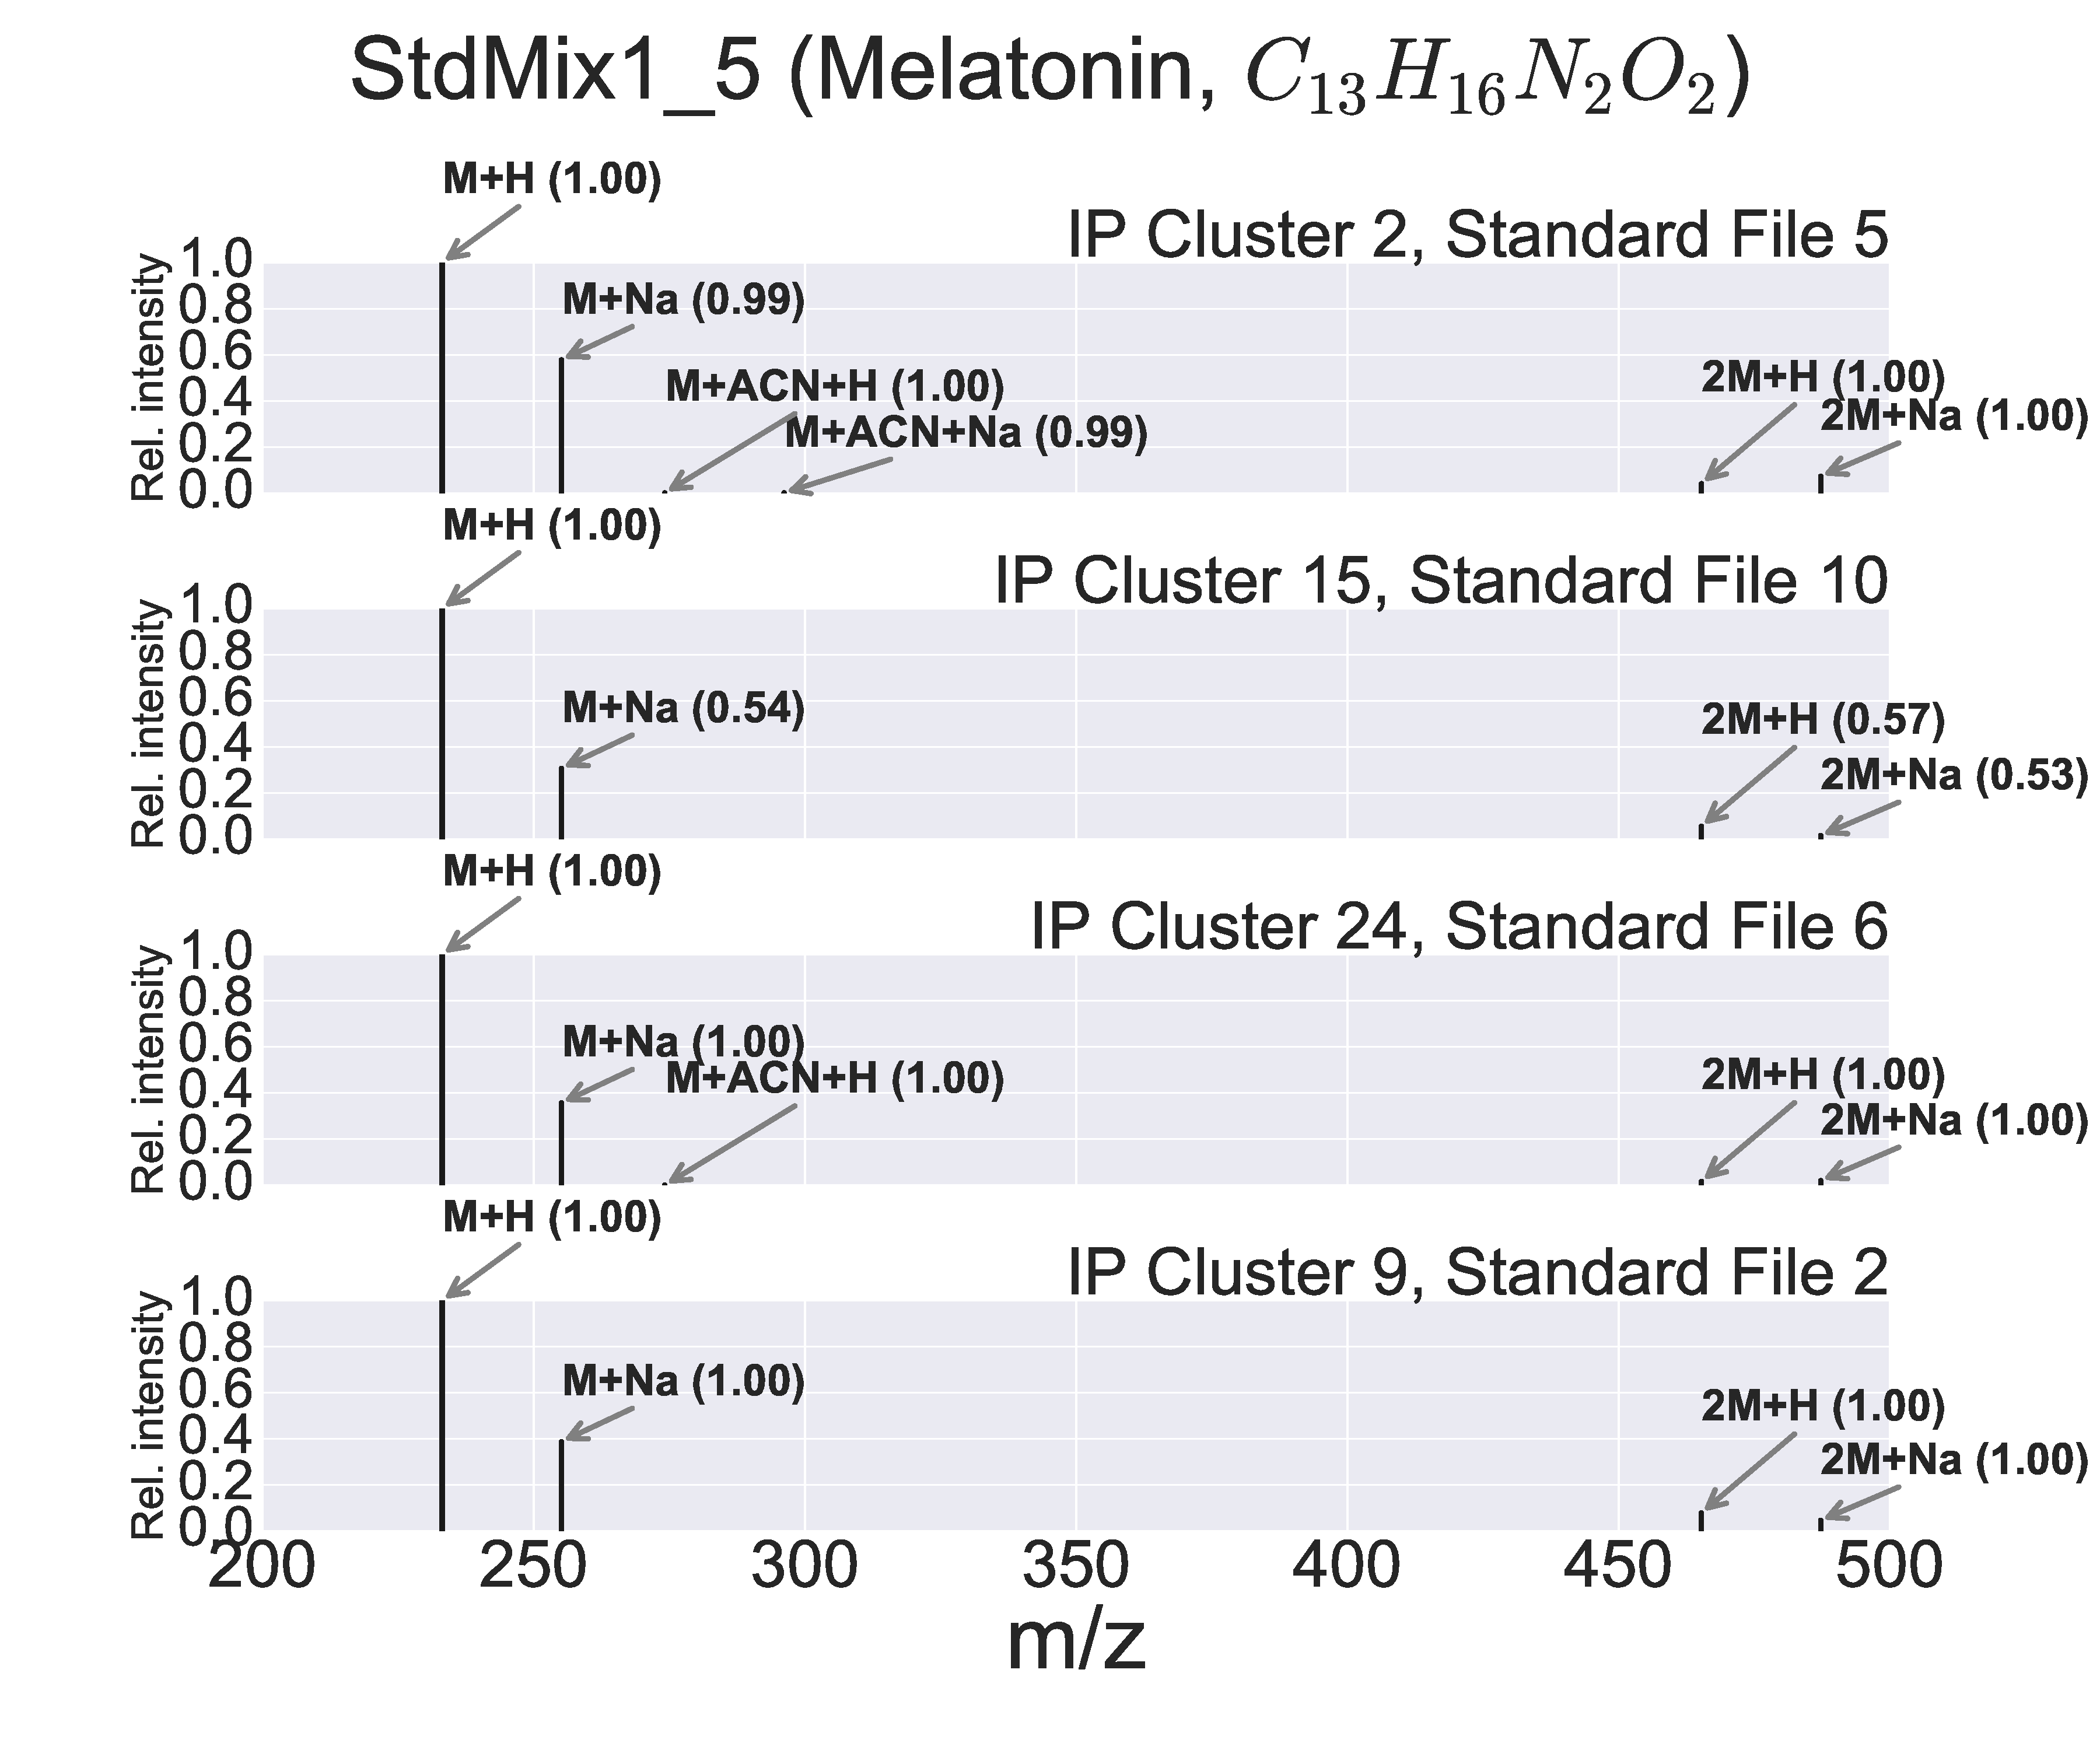
\includegraphics[width=1.0\linewidth]{05-precursor-cluster/figures/melatonin.pdf}
\caption{\label{fig:06} Different IP clusters (2, 15, 24, 9), found in a set of four different Standard runs, which have been putatively identified as corresponding to Melatonin and whose member peaks should therefore be aligned according to the ground truth. Within each run, the first-stage ionization product clustering (PrecursorCluster) gives us the initial assignment of peaks to an IP cluster according to their m/z, RT values and possible transformation types. Here, member peaks are assigned to an IP cluster according to their maximum \textit{a posteriori} probabilities. In the Figure, the posterior transformation type of a peak and its corresponding probability are annotated as a labelled arrow and the bracketed number beside. Across runs, the second-stage clustering (Cluster-Cluster) brings similar IP clusters together, producing an alignment result. The probability of the four peaks $[M+H]^+$ peaks in the Figure to be matched together into a single aligned peakset is 0.87 when the adduct fingerprint term is used and 0.45 without. }
\end{figure}

% \FloatBarrier

\subsection{Running time}

The first-stage clustering of PrecursorCluster is performed independently for each run. In practice, many peaks have no possible transformation except to its own candidate cluster and as such, not all peaks have to be resampled during inference via Gibbs sampling. This allows for efficient inference. On the Standard runs, where each input run may consist up to 5000 peaks, approximately fewer than a quarter of those peaks have to be reassigned. A similar observation can be concluded for the Beer data as well. Taking 10000 posterior samples for each run, Gibbs sampling took approximately 20 minutes per Standard run on our desktop machine (Intel Core i5, 3.3GHz with 8GB of RAM). Furthermore, this step can easily be run in parallel as each run is processed independently of the others.

In the next stage of Cluster-Match, IP clusters are considered to be input features used for matching across runs. The approximate matching algorithm (MW) used in Cluster-Match runs in $O(m\, log\, n)$ time, where $n$ and $m$ are respectively the number of vertices and edges in the graph $G$ to be solved. In practice, this translates to a running time of less than a minute for each sets of Standard runs being processed. The alternative second-stage clustering via Cluster-Cluster requires longer time. By taking 1000 samples for the clustering of IP clusters in each top-level bins, the processing of 2 Standard runs takes approximately half an hour. The entire Cluster-Cluster step can also be easily parallelized as each top-level bin can be processed independently of the others.

\section{Conclusion}

In this paper, we have proposed an integrative workflow that performs precursor clustering of related ionization product peaks and uses that clustering information to improve LC-MS peak alignment (as measured by precision, recall and $F_1$-scores). The valuable information extracted from the first-stage clustering process of ionization product peaks, which lies at the heart of our proposed method, can potentially be used to improve other steps in the pipeline too. For instance, the identification of metabolites, which is currently one of the main bottlenecks in LC-MS data processing, can conceivably be improved by operating on IP cluster-level as the objects of interest rather than dealing with individual LC-MS peak features. This way, the large number of LC-MS peak features in a typical untargeted metabolomics study can instead be represented by a smaller number of IP clusters. In a similar manner, our previous work of MetAssign \cite{Daly2014} considers the relationship between adducts and isotopes in producing probabilistic model for the identification and annotation of peak features. However, in MetAssign, LC-MS peak features coming from different runs have to be aligned (matched) first to form a single consensus feature and a database of known compounds have to be provided. The ionization product clustering model (PrecursorCluster) proposed in this paper addresses the problem differently -- by being able to work with LC-MS peak features coming from multiple runs and not requiring such compound library to be provided (only a list of the expected ionization transformation types is required). As future work, a hybrid model can be developed that combines the best aspects of MetAssign and PrecursorCluster, such that the prior information of compounds expected to be present in the sample is used for clustering some peaks as in MetAssign, while other peaks are clustered entirely based on their possible transformations, as what PrecursorCluster is doing. 

Additionally, once the first-stage clustering of ionization product has been created, we have also demonstrated that establishing the alignment of IP clusters across runs can be performed flexibly, while producing alignment results that are generally competitive or outperforms alignment via the matching of LC-MS peak features alone (as in the case of Cluster-Match). This forms the main contribution of this paper. We have also shown how probabilistic matching of aligned peaksets can be extracted from Cluster-Cluster. For practical use of our workflow and as future work, we foresee the need to develop an interactive visualisation module, particularly to aid in the meaningful interpretation of the results from Cluster-Cluster. This would let the user visualizes aligned peaksets together with their matching probabilities and also the ionization product types annotations obtained from the first stage of the workflow. Enhancements to the first-stage precursor clustering model of PrecursorCluster can also be performed by taking into account the chromatographic peak shapes of IP peaks during clustering, and also information on the predicted RT time of metabolites. As our long term goal, a fully-integrated probabilistic LC-MS data processing pipeline that propagates information and uncertainties across the different steps of the pipeline may also be developed, and it is our hope that the ionization product clustering model, the Cluster-Match approach and the Cluster-Cluster model described in this paper may inspire others along this research direction.